\documentclass{report}
\usepackage{hhline}
\usepackage{listings}
\usepackage[font={small,it}]{caption}
\usepackage{amsmath}
\usepackage{mathtools}
\DeclarePairedDelimiter\ceil{\lceil}{\rceil}
\DeclarePairedDelimiter\floor{\lfloor}{\rfloor}
\usepackage{amssymb}
\DeclareMathOperator*{\argmin}{arg\,min} %argmin
\usepackage{wrapfig}
\setlength{\parskip}{1em}
\usepackage{floatrow}
% Table float box with bottom caption, box width adjusted to content
\newfloatcommand{capbtabbox}{table}[][\FBwidth]
\usepackage{caption}
\usepackage{subcaption}
\captionsetup{compatibility=false}
\usepackage[utf8]{inputenc}
\usepackage{multirow}
%%%
\usepackage{booktabs}
\usepackage{color, colortbl}
\definecolor{LightCyan}{rgb}{0.88,1,1}
\usepackage{array}
% For tabulars
\newcolumntype{P}[1]{>{\centering\arraybackslash}p{#1}}

\usepackage{pdfpages}
\usepackage{graphicx}
\usepackage{longtable}
%\usepackage[export]{adjustbox}
%\usepackage{tabu}
\usepackage{xcolor,colortbl}
\usepackage{caption}
\usepackage{subcaption}
\usepackage{float}
\usepackage{wrapfig}
\usepackage{amsfonts}
\usepackage{amsthm}

\usepackage[margin=0.65in]{geometry}
\usepackage{url} % for bibliograpy links

\newcommand{\abs}[1]{\lvert#1\rvert}
\newcommand{\norm}[1]{\lVert#1\rVert}


\begin{document}

\vspace*{3ex}
\begin{flushright}
{\large \today}
\end{flushright}

\vskip20ex
\hskip3cm

\begin{center}


\begin{figure}[H]
\centering
\begin{subfigure}{.5\textwidth}
  \centering
  
\includegraphics[width=.9\linewidth]{images/mini.png}
\end{subfigure}%
\begin{subfigure}{.5\textwidth}
  \centering
  
\includegraphics[width=.9\linewidth]{images/pw.jpg}
\end{subfigure}
\end{figure}




\Large {\bf
	Bachelor Thesis \\
	Simulation of Movement of a Ship Floating on Water Surface
}

\Large {\bf 
Author: Bartłomiej Dybisz 
}

\Large {\bf 
Supervisor: mgr inż. Paweł Aszklar
}
\end{center}
\vskip2ex


\vskip25ex



\newpage
\tableofcontents
\newpage


%------------------------------------------------------------------------------
\section*{Schedule}

\begin{center}


\begin{table}[h]

\large
\begin{tabular}{|l|l|l|}
\hline
\multicolumn{3}{|l|}{\cellcolor[HTML]{C0C0C0}Schedule} \\ \hline
Date         & Note        & Planned Progress          \\ \hline
\hline

22.04.2016   &     & Presentation of Business Analysis.   \\ \hline
25.04.2016   &     & Additional changes in Business Analysis.   \\ \hline
10.05.2016   &     & Presentation of Water Module.   \\ \hline
17.05.2016   &     & Presentation of Technical Project. \\ \hline
24.05.2016   &     & Additional changes in Technical Project.  \\ \hline
07.06.2016   &     & Presentation of Ship Module.  \\ \hline
13.06.2016   &     & Presentation of GUI Module.  \\ \hline
14.06.2016   &     & Complete system.  \\ \hline

\end{tabular}
\end{table}

\end{center}

%---------------------------------------------------------------
\newpage
\chapter{Business Analysis}
\section{Glossary}
\begin{itemize}
\item \textbf{Computer Simulation} is the discipline of designing a model of an actual or theoretical physical system, executing
the model on a digital computer, and analyzing the execution output. Simulation embodies the principle of
“learning by doing” — to learn about the system we must first build a model of some sort and then operate the
model \cite{gloss_1}.
\item \textbf{Graphics Pipeline} The graphics pipeline in a fundamental concept in computer graphics and refers to a series of
interconnected stages through which data and commands describing a scene go through when being rendered \cite{gloss_2}.
The basic functionality of the graphics pipeline is to transform your 3D scene, given a certain camera position and
camera orientation, into a 2D image that represents the 3D scene from this camera’s viewpoint \cite{gloss_3}.
\item\textbf{User Interface} In information technology, the user interface (UI) is everything designed into an information device
with which a human being may interact - including display screen, keyboard, mouse, light pen, the appearance of
a desktop, illuminated characters, help messages, and how an application program or a Web site invites interaction
and responds to it \cite{gloss_4}.
\item \textbf{Skybox} is a panoramic texture drawn behind all objects in the scene to represent the sky or any other vista at a
great distance \cite{gloss_5}.
\item \textbf{Heightmap} A two-dimensional raster image used to store surface elevations that can later be applied to a threedimensional
object \cite{gloss_6}. Classic approach involves storing height values in particular channel of an image and using
them to elevate grid’s vertices.
\item \textbf{Camera} is a series of transformations, which in the end convert an object from three dimensional space to two
dimensional pixels. Standard process involves model, view, projection and viewport transformations, which are
usually represented in form of matrices.
\end{itemize}

\section{Goal}
The main goal of this project is to deploy application, which will constitutes a decent simulator of a ship on a water surface. The application should demonstrate interactive environment and be able to cope with modeling both, a boat and a water in real time. The program will serve as a basis for a sailboat-based video game and its functionalities will
have great impact on releasing the title.

To start with, the scene should be bounded by a textured cube - a skybox. The box will imitate surroundings preventing graphics pipeline from rendering redundant elements of the environment. Computational power should be focused on the simulation itself. The user must be allowed to freely explore the scene with usage of a controller.

The water surface should be interactive in a sense that user will be able to produce a disturbance. It can be e.g. achieved via mouse click. As the supplemental feature one may consider introducing some constant interfere of the surface like e.g. rain. It is vital for the project that water will act like a medium size body. A lake or a pool is an accurate illustration. Any types of breaking waves are dispensable. Rendering the surface should consider reflection and refraction along with Fresnel’s coefficient.

The ship must react to the water changes to such extent that it is possible for him to flip. It is suggested that boat’s model should be independent from the algorithm, but it is not essential. Vital part of the simulation though, is ship’s steering - one should be able to force the craft to move around with e.g. keyboard usage. Of course the movement must
be affected by the surrounding water.

Last but not least, the application should provide user interface with as many modifiable parameters as possible. Changes in variables must have instant impact on the simulation without any need for restart. Since application will be of use not only for programmers, interface is the program’s inevitable part.

\section{User Stories}
As a user I want to:
\begin{itemize}
\item be able to freely move around the scene.
\item zoom the animation.
\item disturb water surface in a particular point.
\item control the ship’s movements.
\item change parameters related to the water simulation.
\item change parameters related to the ship simulation.
\item close the application.
\end{itemize}

\section{Functional Requirements}
In all tables of the following section we assume that priority can take following values:
\begin{itemize}
\item 1 - must be implemented
\item 2 - can be implemented optionally
\item 3 - is a nice addition, but not essential.
\end{itemize}

\begin{center}
\hspace*{-2.1cm}
	\begin{longtable}{| l | p{4cm} | p{3.5cm} | l |}
	
		\hline
	  	ID & Requirement & Comments & Priority \\
		\hline
		
		1 & 
		Camera movement must be intuitive and allow to access every part of the simulation
 & Although combination of mouse end keyboard is preferred, one could introduce different approach.
		 &
		1 
		\\ \hline
		
		2 & 
		Water must be prone to disturbance in a particular point of its surface. & As before, developer can choose a form of user interaction.
		 &
		1 
		\\ \hline		
	
		2.1 & 
		User should be able to choose the level of disturbance. Higher the level, bigger the waves. & Nice addition to the interface 
		 &
		2 
		\\ \hline		
	
			2.2 & 
		Accuracy of water surface in terms of the number of quads can be modified. & Excellent part of the interface. 
		 &
		2 
		\\ \hline		
		
		2.3 & 
		Accuracy of the simulation algorithm can be tweaked.
& For example different numerical approaches can be set.

		 &
		3 
		\\ \hline			

		2.4 & 
		Different types of constant water disturbance like e.g rain& Can be added to the interface as a list of choices
		 &
		3 
		\\ \hline		

		3 & 
		Ships steering controlled by the user.&  Keyboard suggested.
		 &
		1 
		\\ \hline	

		3.1 & 
		Position of the ship can be dynamically changed.
& If one wants e.g. start again in some particular point
		 &
		2
		\\ \hline	
	
		3.2 & 
		Current ship’s vital parameters (e.g. buoyancy point, current position, acting forces) displayed in the interface. & 
		 &
		2 
		\\ \hline		
		

		3.3 & 
		Additional projection displaying 2D intersection of the ship and its level of immersion. & 
		 &
		3
		\\ \hline		


		4 & 
		The animation can be stopped at any point  & Useful in debugging
and evaluating rendered scene

		 &
		2
		\\ \hline
	
		4.1 & 
		A fog with controlled intensity& 
		 &
		3
		\\ \hline	

		4.2 & 
		Light source with its position and intensity parametrized. & 
		 &
		3
		\\ \hline

		4.3 & 
		Some general sounds of a water and environment. & 
		 &
		3
		\\ \hline
	
		4.4 & 
		Ability to load and save the settings. & E.g. config.ini file located in the same directory as executable
		 &
		2
		\\ \hline
		
		4.5 & 
		Loading arbitrary model as a ship. & 
		 &
		3
		\\ \hline
		
		4.6 & 
		Clicking ’X’ button must close the application
 & 
		 &
		1
		\\ \hline	
		
	\end{longtable}
\end{center}

\section{Non-Functional Requirements}
\subsection{Reliability}
The simulator is expected to reduce number of glitches and malfunctions of the rendering and simulation process to the minimum. One should avoid situations where e.g. ship has stuck to the wave and is not controllable or water is slowly moving up. Vital point is the accuracy of the algorithm - water must look convincing with 60 fps conserved.

What is more, user interface should interact with the scene without any problems. Modifying a parameter must ad hoc impact the scene and values that are not permitted must be unprocessed by the program.

\subsection{Performance}
The application must work in real time i.e. 60 frames per seconds in average must be kept. Following assumption must be true only for the default parameters and their small deviations - if one wants to provide some enormous number of triangles to render, he is free to do so, but can not expect smooth performance. The parameters are assumed to provide
water grid of edge size equal to 32 and 256 vertices per side.

The program obviously assumes minimal hardware and software requirements: Windows 7 64bit, 3GB RAM, dedicated graphics with OpenGL 3.3 or DirectX 9.0c, Intel Core I3 2.13 GHz.

\subsection{Security and Safety}
No internal or external threats.

\subsection{Risk Analysis}
One should consider adjusting algorithm of water/ship simulation to the real time demands of the project as the main risk. There is no denial that spending too much time on tweaking the algorithm that cannot cope with the performance assumptions, will delay work and may cause one to neglect the application’s crucial parts. It is then advisable to implement well known algorithms of rather small complexity at the beginning and proceed with other functionalities. When all of them will be met, one could start increasing accuracy and robustness of the modeling process via introducing
some more complicated algorithms.

In addition, since user interface is a feature that should be developed along with other parts of the project, one might
consider shorter time destined to focus on this module alone


%---------------------------------------------------------------
\newpage
\chapter{Technical Analysis}
\section{Introduction}
Following work comprises a technical approach to the problems stated in the business analysis. It tries to cope with various algorithms related to the simulation and, if needed, presents their mathematical derivations. One will start with short presentation of the production model (section \ref{sec:production_model}), followed by summary of used technology (section \ref{sec:technology}).

Section \ref{sec:algorithms}, will bring core of the paper - the algorithms. Preceded by brief notes about mathematical notation (subsection \ref{subsec:math_notation}), scene setup along with water and ship representations will be shown. All three, outline general composition of the application and provide a foundation for further topics. In addition, basic computer graphics transformations used in the system are listed in subsection \ref{subsec:basic_transform}. Since they are assumed to be known, their appearance is dictated solely by section \ref{subsec: disturbing_water}, where disturbance of the water's grid will be demonstrated. One will get to know about conversion from screen coordinates to the world coordinates in purpose of finding a ray's crossing point with a plane. What is more, straight forward procedure for localizing intersected vertex will be given. Next, one will face subsection \ref{subsection:water_shading}, which will tackle the algorithm for coloring the water. Raised issues include, but are not limited to, reflected and refracted rays, ray-box intersection and Fresnel's coefficient approximation. Last but not least, there are two subsections devoted to the process of simulating the physical phenomena. First one (subsection \ref{subsec:water_simulation}), will start with an overview of the system's internal structure for updating the water's grid. One must note that it involves terminology related strictly to the OpenGL API, namely: frame buffer objects and textures. To provide better understanding of used numerical algorithm, the section additionally contains its mathematical derivations. Starting from elemental derivative formula, one can follow the full path to approximation of partial derivatives in the considered equation. On the other hand, subsection \ref{subsec:ship_simulation} are dedicated entirely to methods that concerns the simulation of the ship. One can acquire the knowledge of computing the buoyancy center and buoyancy force of the immersed boat's hull, based on precomputed, three dimensional grid. Both will enable PhysX libary to estimate transformations of the ship in each time frame. In addition, subsection \ref{subsub:physX} will present a general sketch of calculations that happen behind the scenes of the library. One may find it useful in case of a need of extending the project's functionalities.

Although not a single line of code appears in the paper, class diagrams of the system's architecture are available in subsection \ref{sec:model}. The section will also provide terse descriptions of provided graphs, helping one to grasp the main functionalities of the design. 


%---------------------------------------------------------------
\section{Production Model} \label{sec:production_model}
The section is rather brief. It starts with short introduction to the scrum terminology and without redundant details, every important roles of the approach are presented. Next, one can read why Scrum has been chosen and how it has been adapted to shipping the product. The section ends with the list of tasks (along with dates of their completion) needed to build the project; Table \ref{tab:product_backlog}.

\subsection{General Information}
According to \cite{scrum_definition}, Scrum is an iterative and incremental framework for project management mainly deployed in agile software development. The scrum methodology emphasizes functional software, the flexibility to change along with emerging business realities, communication and collaboration. It consists of:
\begin{itemize}
\item \textbf{Product Backlog}

Is an ordered list of user stories that may be implemented in the shipped product. It is also the single source of the product's features, functions, requirements etc. 

\item \textbf{Product Owner}

The Product Owner is in charge of the backlog's content as well as redistributing tasks over consecutive sprints.

\item \textbf{Sprint}

The heart of Scrum; a time-box of one month or less during which a “Done”, useable, and potentially releasable product Increment is created \cite{scrum_guide}. Sprint includes user stories, which are a subset of the Product Backlog. Normally, sprints happens one after another, creating continued work flow. 

\item \textbf{The Development Team}

Consists of professionals who realizes a sprint. They implement and test desired user stories.

\item \textbf{Scrum Master}

The Scrum Master is responsible for ensuring Scrum is understood and enacted. Scrum Masters do this by ensuring that the Development Team and Product Owner adheres to Scrum theory, practices, and rules \cite{scrum_guide}.

\item \textbf{Daily Scrum}

The Daily Scrum is a 15-minute time-boxed event for the Development Team to synchronize activities and create a plan for the next 24 hours. This is done by inspecting the work since the last Daily Scrum and forecasting the work that could be done before the next one \cite{scrum_guide}. 

\end{itemize}

To even better grasp the idea, Figure \ref{fig:scrum_diag} has been composed. On its left hand side one can observe the Product Backlog, filled up with different user stories that needs to be completed. Next frame depicts assigning some of user stories to a particular sprint. As top buckles suggest, it is the place where Product Owner and Development Team meets. First one moves tasks from Product Backlog to Sprint Backlog, and the latter one starts to implementing them. During next 2 to 4 weeks the team creates a stand-alone piece of the Goal Product, using Daily Scrums as a tool for overseeing the work. Goal product is based on multiple parts - each created by separate sprint, hence when not all of them were supplied, another sprint must be organized. In addition, because each part of the Goal Product works independently, the production cycle can be stopped at any time with certainty that the product will be functional (but not necessary completed). Since the Scrum Master may influence every aspect of Scrum methodology, the figure deliberately omits it. One should note that the diagram rather lacks of precision in order to present the general idea. Because of that it cannot be treated as a full description of the Scrum approach.

\begin{figure}[H]
    \centering
    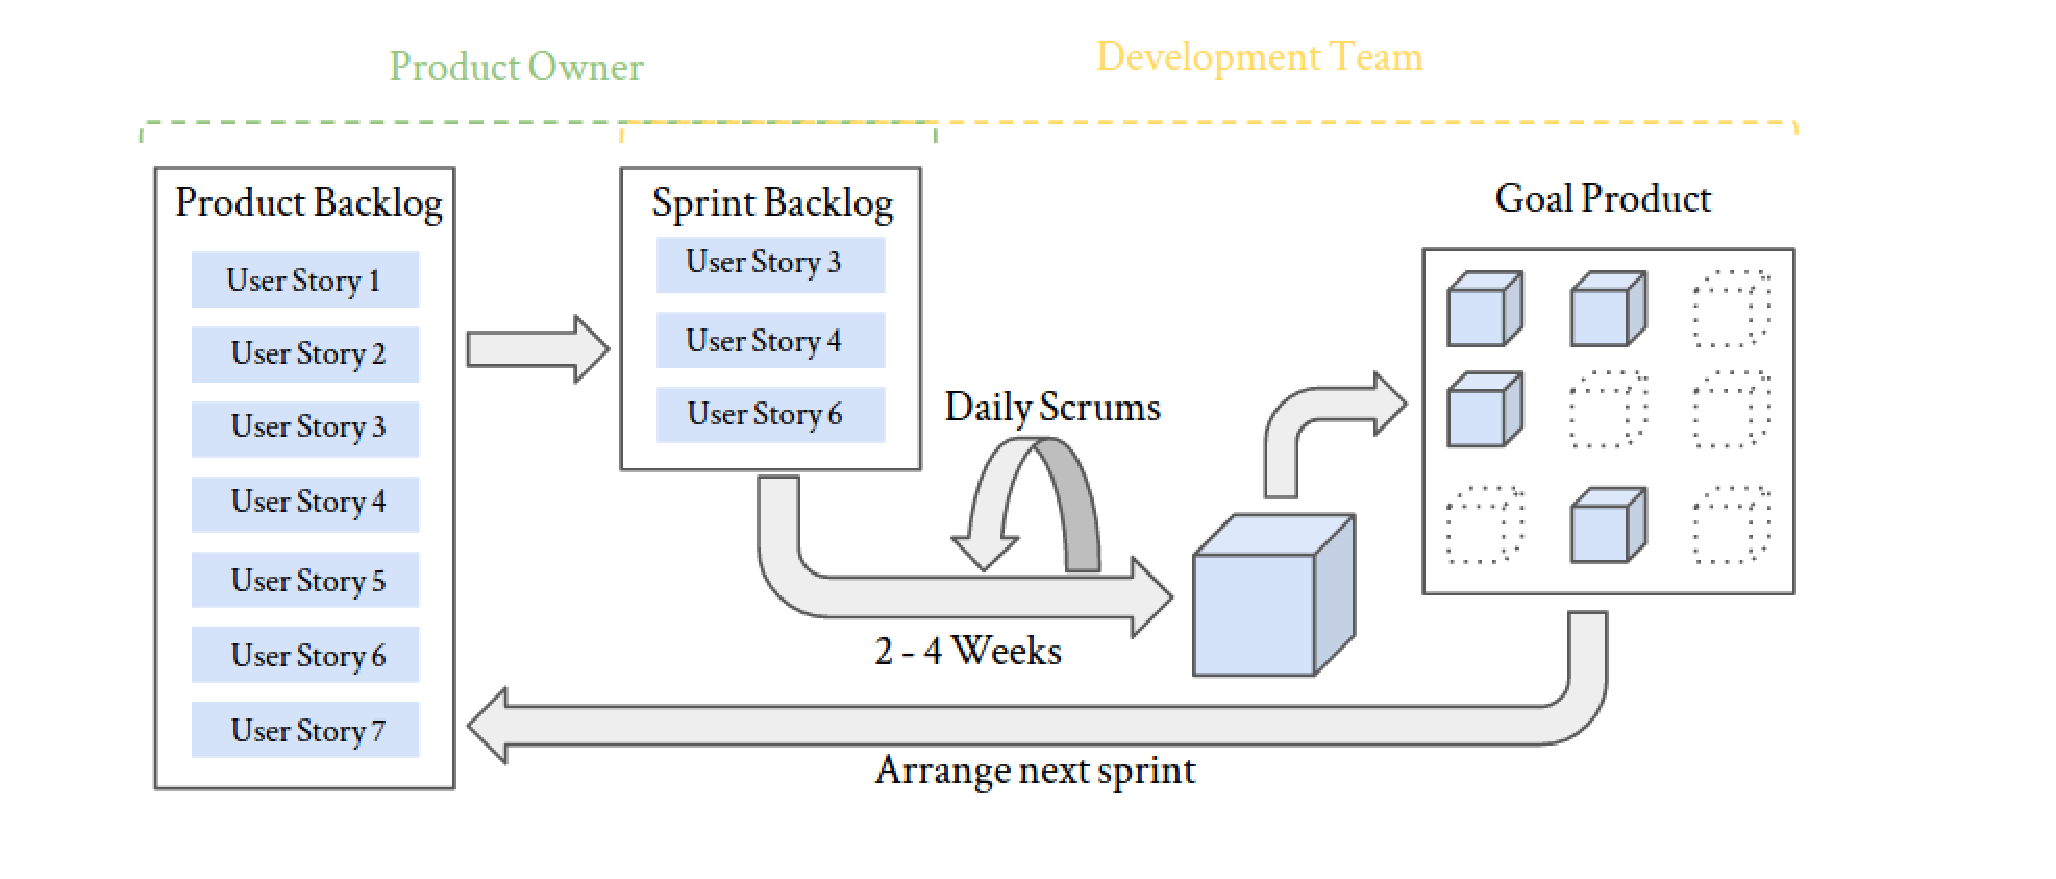
\includegraphics[width=0.8\textwidth]{images/scrum_diag.pdf}
    \caption{General overview of the scrum methodology.}
    \label{fig:scrum_diag}
\end{figure}

\subsection{Adaptation to the Project}

What is really interesting  though, is its presume that stand alone parts of the goal application  are developed and tested over specified time interval (during sprints). Such an approach fits perfectly to the project's characteristics and seems to be the only advantage over other methodologies. Because of the nature of following project (one-man's work), roles of: Scrum Master, Product Owner and Developer Team will be assign to the author. Obviously, Daily Scrum will not be needed and the burndown chart of the work will be included in the final thesis document.

Since user stories provided by the business analysis are small set of general ideas, the paper will split them into smaller pieces. It will help to estimate total amount of time needed to complete each sprint, as well as clarify the specific objectives. Table \ref{tab:product_backlog}, represents a mix of Product and Sprint Backlog. As mentioned, user stories were divided into smaller tasks and assigned to particular sprints. Each task has estimated number of days needed to its completion. Overall interval has been provided to give an overview of the development process.

\begin{longtable}{| p{.20\textwidth} | p{.50\textwidth} | p{.05\textwidth}| p{.05\textwidth}|  p{.10\textwidth}|} 
\hline
User Story  & Task & Days & Sprints & Interval\\ \hline

\multirow{5}{80pt}{As a user I want to be able to freely move around the scene.} & Create a window with OpenGL context. &2 & \multirow{5}{80pt}{1}  &\multirow{5}{80pt}{01.04.2016 \\ 24.04.2016}\\\cline{2-3} 
 & Handle keyboard and mouse input/output. &2 & &\\\cline{2-3}
 & Display the skybox with arbitrary texture. &4& &\\ \cline{2-3}
 & Display flat water grid with shading.&14& &\\ \cline{2-3}
 & Camera control.&2 &&\\\cline{2-2} \hline
 
 \multirow{5}{80pt}{As a user I want to disturb water surface in a particular point.} & Find intersection point with the water's grid.&2 & \multirow{5}{80pt}{\\2} & \multirow{5}{80pt}{25.04.2016 \\ 10.05.2016}\\ \cline{2-3}
 & Disturb water at a given point &1 && \\ \cline{2-3}
 & Disturb water's area around the given point. &1& & \\\cline{2-3}
 & Random disturbances along the water's grid (e.g. rain). &1& & \\\cline{2-3}
 & Off-screen calculations for simulating the waves. &5& & \\\cline{2-3}
 & Deform the water's grid according to waves equations. &5 && \\\cline{2-3} \hline
 
 \multirow{4}{80pt}{As a user I want to control ship's movements.} & Load and render model of the ship.&2 & \multirow{4}{80pt}{\\3} & \multirow{4}{80pt}{11.05.2016 \\ 19.05.2016}\\ \cline{2-3}
 & Move ship around the scene. &3& & \\ \cline{2-3}
 & Display ship's boundary grid. &1& & \\\cline{2-3}
 & Calculate the grid's cell that are over/under the water's grid. &2 && \\\cline{2-3} \hline
 
  \multirow{5}{80pt}{As a user I want to experience influence of the waves on ship's hull.} & Compute gravitational center point of the ship. &2& \multirow{5}{80pt}{\\4} & \multirow{5}{80pt}{20.05.2016 \\ 14.06.2016}\\ \cline{2-3}
 & Compute buoyancy point of the ship. &2& & \\ \cline{2-3}
 & Compute moment of inertia tensor. &7 && \\\cline{2-3}
 & Calculate forces acting on the ship. &11 && \\\cline{2-3} 
  & Apply forces to the model of the ship. &2 & &\\\cline{2-3}\hline

  \multirow{5}{80pt}{As a user I want to tweak the application's parameters.} & User interface for the general scenes parameters.&1 & \multirow{5}{80pt}{\\5} & \multirow{5}{80pt}{15.06.2016 \\ 22.06.2016}\\ \cline{2-3}
 & User interface for the water's parameters. &1 && \\ \cline{2-3}
 & User interface for the ship's parameters. &1 && \\\cline{2-3}
 & Loading configuration files. &2 && \\\cline{2-3} 
  & Unit tests. & 2&& \\\cline{2-3}\hline 
 
 
\caption{Product/Sprints backlog of the ship simulator. It depicts all tasks that need to be completed in order to successfully finish the project.}
\label{tab:product_backlog}
\end{longtable}




%---------------------------------------------------------------
\section{Technology} \label{sec:technology}
Technology chosen to accomplish the ship's simulator should not be a surprise for anyone. Open Graphics Library (OpenGL) has been seleted to handle the rendering. Since it is widely used standard in various computer graphics fields, it was only a natural choice. In a nutshell, the library constitutes a cross-platform application programming interface (API), written entirely in \texttt{C} language, that interacts with graphics processing unit (GPU) to achieve hardware-accelerated rendering of 2D and 3D vector graphics. Along with a means for display the scene one should provide a library to perform computations related to the physical simulations. For the project purposes, widely known and recommended NVIDIA's PhysX library has been chosen. According to the developer's page: it is a scalable multi-platform game physics solution supporting a wide range of devices \cite{physx}. Next, due to great memory management and object orientation, \texttt{C++} has been chosen as the main programming language. What is more, its straight-forward compatibility with OpenGL API and PhysX is rather indispensable. As the central tool to control compiling and linking process, CMake was pegged. It is a great free and open-source software to managing the build process. Numerous external libraries take part in the application flow. Following list summarizes them all:
\begin{itemize}
\item \textbf{Ant Tweak Bar}

Small and easy-to-use C/C++ library that allows programmers to quickly add a light and intuitive graphical user interface into graphic applications based on OpenGL (compatibility and core profiles), DirectX 9, DirectX 10 or DirectX 11 to interactively tweak parameters on-screen \cite{anttweakbar}.

\item \textbf{Simple OpenGL Image Library (SOIL)}

is a tiny C library used primarily for uploading textures into OpenGL. It can also be used to save and load images in a variety of formats (useful for loading height maps, non-OpenGL applications, etc.) \cite{soil}.
\item \textbf{The OpenGL Extension Wrangler Library (GLEW)}

is a cross-platform open-source C/C++ extension loading library. GLEW provides efficient run-time mechanisms for determining which OpenGL extensions are supported on the target platform \cite{glew}.
\item \textbf{GLFW}

is an Open Source, multi-platform library for creating windows with OpenGL contexts and receiving input and events \cite{glfw}.
\item \textbf{OpenGL Mathematics (GLM) }

is a header only C++ mathematics library for graphics software based on the OpenGL Shading Language (GLSL) specifications \cite{glm}.
\item \textbf{INI Not Invented Here (INIH)}

is a simple .INI file parser written in C. It's only a couple of pages of code, and it was designed to be small and simple, so it's good for embedded systems \cite{inih}.
\end{itemize}
Although all technologies picked to create the application allow cross-platform development, its target platform is Windows. 



%---------------------------------------------------------------
\section{Algorithms} \label{sec:algorithms}
The central theme of the following section are algorithms developed to achieve business analysis requirements. Text will focus mainly on presenting mathematical formulas and their derivation rather than specific implementations. In some segments objects characteristic for OpenGL will be introduced to fully cover particular concepts. Before one will begin, one is encouraged to familiarize with mathematical notation assumption. 

\subsection{Mathematical Notation} \label{subsec:math_notation}
To provide more transparent source of reference, instead of a block of text, table will be presented. As always, the simplicity should works in favour of the array, hence it consists only of two columns. First one presents examples of notation, while the second one descriptions.

\begin{longtable}{| p{.20\textwidth} | p{.40\textwidth} |} 
\hline
Example  & Description \\ \hline
$\vec{v}$& vector $v$ \\ \hline
$M$ & matrix $M$ \\ \hline
 $\norm{\vec{v}}$ & magnitude of vector $v$ \\ \hline
 $a\cdot b$ or $ab$ & elemental multiplication \\ \hline
 $\circ$ & dot product, namely $\vec{v_1} \circ \vec{v_2} = \norm{\vec{v_1}} \cdot \norm{\vec{v_2}} \cdot \cos(\theta)$, where $\theta$ is an angle between the two vectors. \\ \hline
$\vec{u} \measuredangle \vec{v}$ & an angle between vectors $u$ and $v$ \\ \hline

$\floor{a}$ & where $a \in \mathbb{R}$, represents the floor function i.e. it will return only integer part of $a$'s value \\ \hline

$f'(x) = \frac{df(x)}{dx}$ & a derivative of function $f$ in point $x$.\\ \hline
$\frac {\partial{^2f}}{\partial t^2}$ & a partial derivative of function $f$ \\ \hline

\caption{List of mathematical notation used through out the paper.}
\label{tab:product_backlog}
\end{longtable}

Any other notations will be understandable via their descriptions or from a context. One should note that there is no special indication for a point.

\subsection{Scene Setup} \label{subsec:scene_setup}
Although it is distantly interrelated with algorithms, scene setup does include some mathematical concepts which need to be addressed. First of all, one should take a look at Figure \ref{fig:scene_setup}. It presents the scene consisting of:
\begin{itemize}
\item \textbf{Water Surface}

Represented by square, $n \times n$ grid of size $a$, where $n$ represents a number of vertices per side. Its center is located at the origin of the world coordinates. When not disturbed, the grid lies entirely on $XZ$ plane, slicing the cube. 

\item \textbf{Skybox}

A texturized cube, of size $a$. Its center is also located in the origin of the worlds coordinates. In some sense it constitutes the scene's boundary, hence it is treated as a impassable border for the ship model.

\item \textbf{Ship}

A model of the ship that will be simulated. 

\end{itemize}


\begin{figure}[H]
    \centering
    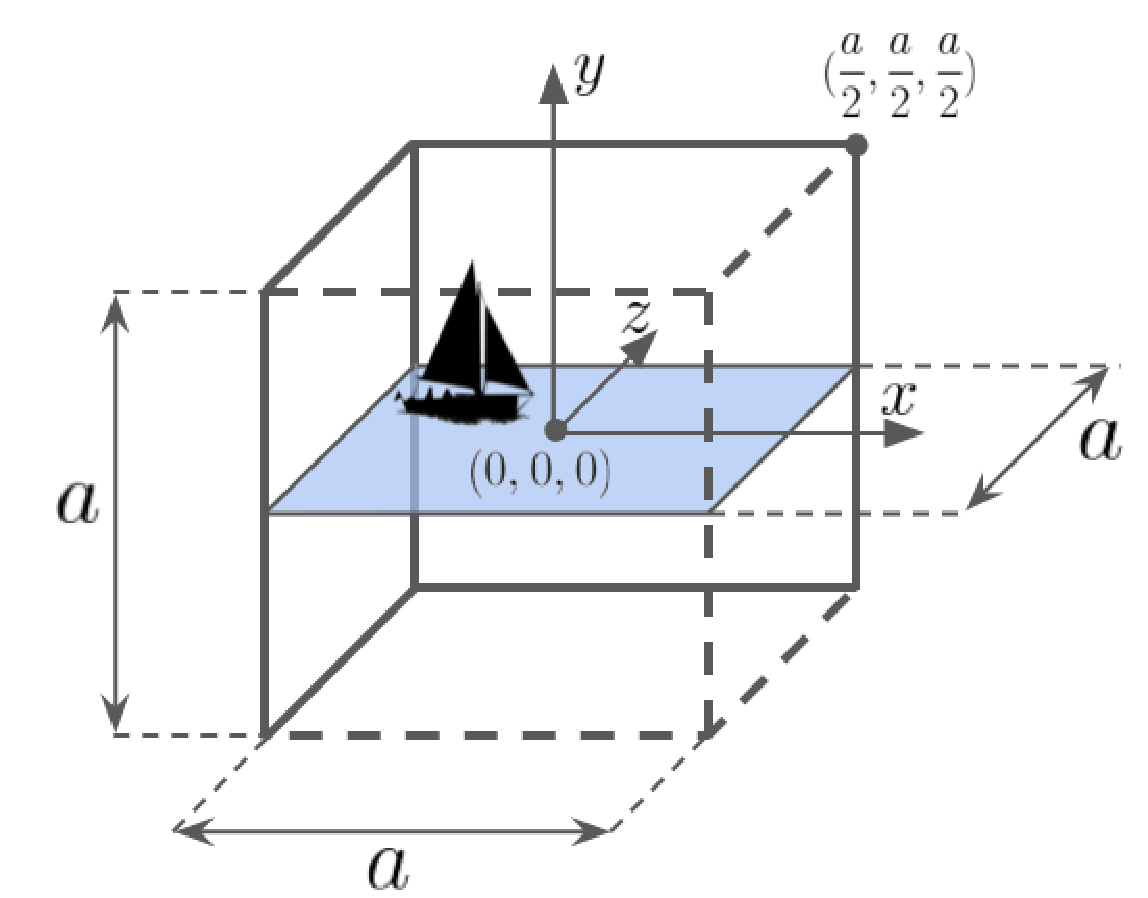
\includegraphics[width=0.3\textwidth]{images/scene_setup.pdf}
    \caption{General overview of the scene setup.}
    \label{fig:scene_setup}
\end{figure}

\subsection{Water Representation} \label{subsec:water_repr}
The water surface will be implemented as a grid of vertices. Each 4 neighboring vertices will form a quad. Quad consists of two right angled triangles, which shares hypotenuse. With following setup the grid will be treated as a height field. As a consequence, its vertices will change values only along $Y$ axis. Figure \ref{fig:water_deform} depicts example of a water grid in two states: stable and with random disturbance. Although it may seem like a serious drawback, it suits well the business analysis' assumption about no breaking waves. What is more, as shown further in the paper, it allows almost 1-1 projection onto the texture object, which is needed for numerical approximation to compute.

\begin{figure}[H]
\begin{subfigure}{.5\textwidth}
  \centering
  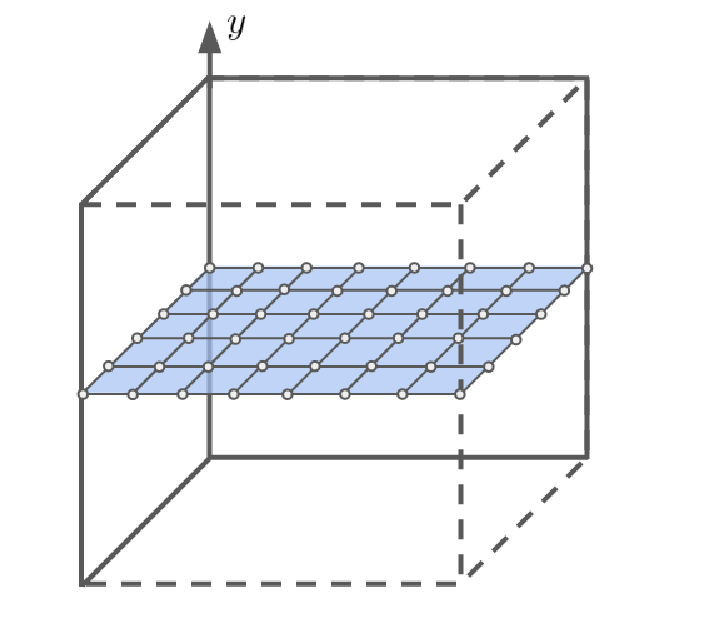
\includegraphics[width=.6\linewidth]{images/water_grid_stable.pdf}
  \caption{Undisturbed water grid in the scene.}
  \label{fig:sfig1}
\end{subfigure}%
\begin{subfigure}{.5\textwidth}
  \centering
  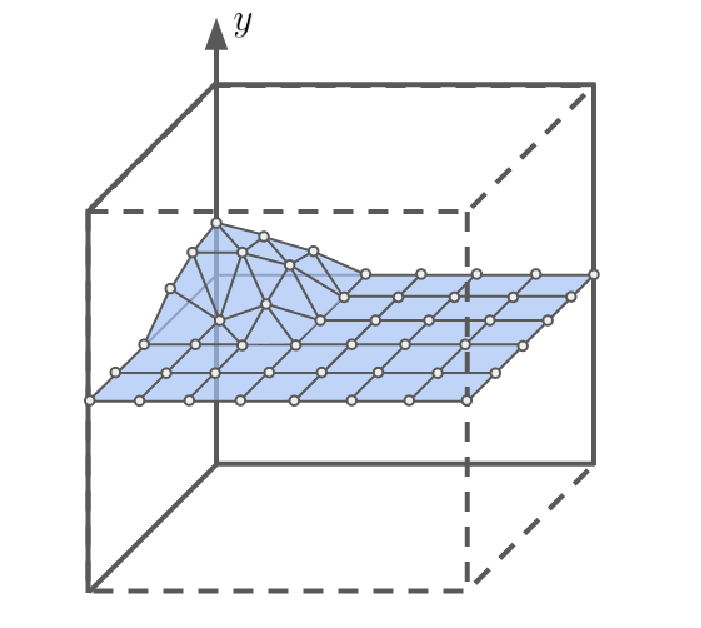
\includegraphics[width=.6\linewidth]{images/water_grid_disturbed.pdf}
  \caption{Random disturbance in the water's grid.}
  \label{fig:sfig2}
\end{subfigure}
\caption{Plots of water grid in two different conditions.}
\label{fig:water_deform}
\end{figure}

\subsection{Ship Representation} \label{subsec:ship_repr}
The ship will be represented using Wavefront .obj file. It is nothing more than a specific file format, which allows storing data that represents 3D geometry solely. Since the application does not require animation of a model, the format satisfies buisiness analysis demands. Figure \ref{fig:ship_obj} depicts a model that will be used during code production and the application testing. It is a small fishing boat with low number of vertices to prevent long loading time. The model has been acquired completely free from the \cite{boat_source}. One should note that the model in the final application will differ in order to present more complex shape and make the scene more pleasant to the eye. What is more, within the application's sources the class with ability of loading arbitrary .obj models will be shipped. One can find it useful in case of morphing the project into a game.


\begin{figure}[H]
\begin{subfigure}{.3\textwidth}
  \centering
  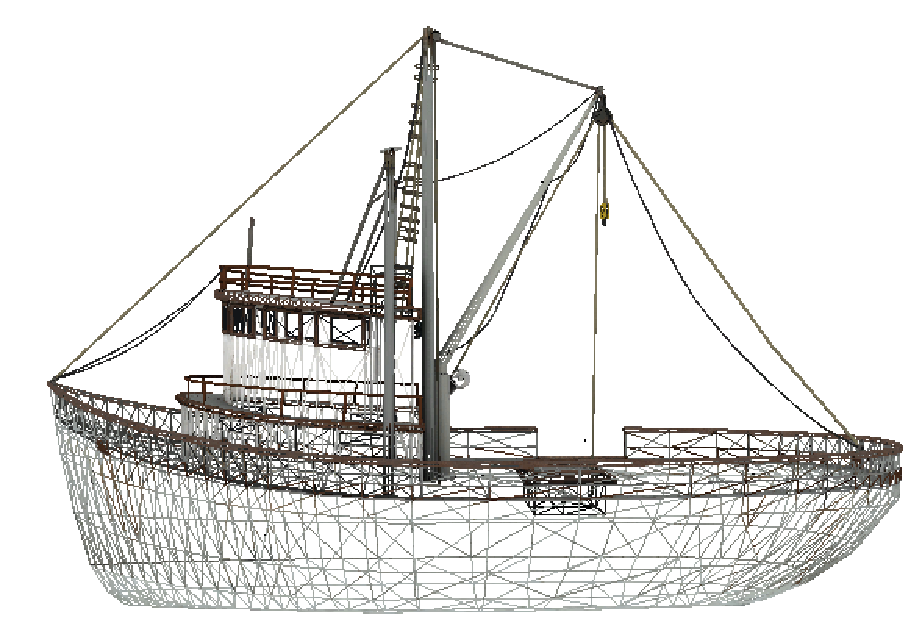
\includegraphics[width=.8\linewidth]{images/ship_sketch_1.pdf}
  \label{fig:ship_sketch_1}
\end{subfigure}%
\begin{subfigure}{.3\textwidth}
  \centering
  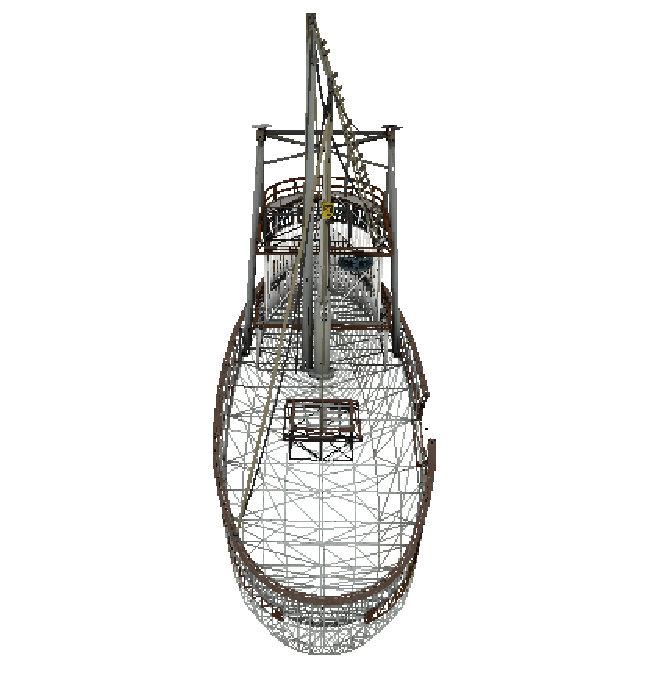
\includegraphics[width=.8\linewidth]{images/ship_sketch_2.pdf}
  \label{fig:ship_sketch_2}
\end{subfigure}
\begin{subfigure}{.25\textwidth}
  \centering
  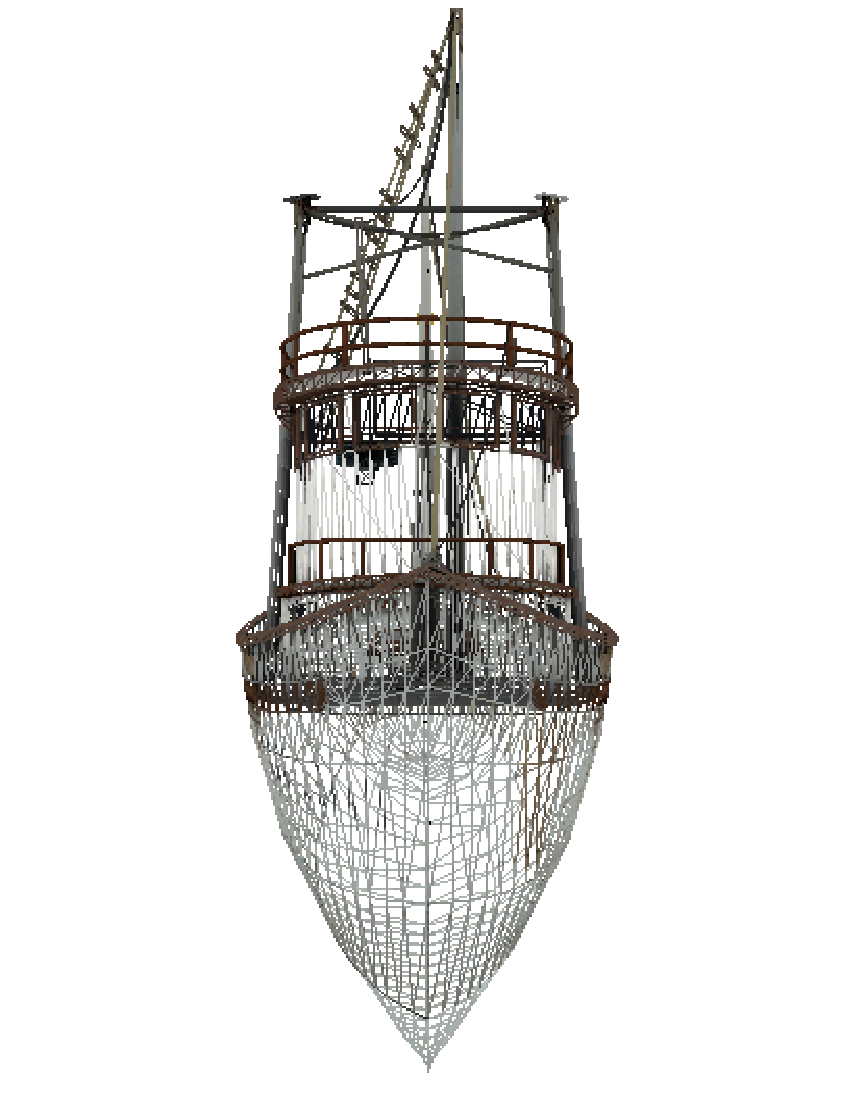
\includegraphics[width=.8\linewidth]{images/ship_sketch_3.pdf}
  \label{fig:ship_sketch_3}
\end{subfigure}
\caption{The model used in the simulation. It is a small fishing boat with low number of vertices.}
\label{fig:ship_obj}
\end{figure}

\subsection{Basic Transformations} \label{subsec:basic_transform}
The section briefly describes vertices transformations in a rendering pipeline. If one does not know anything about the matter, he or she is encourage to fill that knowledge gap to help understand concepts presented in Section \ref{subsec: disturbing_water}. Note that words: coordinates and space are used interchangeably. 

When rendering a scene in 3D space, there are usually 3 transformations that are applied to the 3D geometry in the scene:
\begin{itemize}
\item \textbf{Model Matrix $M$}

Transforms a models vertices from object space (local frame of reference visible e.g. during creation of 3D models in various tools like Blender or Maya) into world coordinates (also called world space). World coordinates is the position, orientation (and sometimes scale) that positions the model in the correct place in the world.

\item \textbf{View Matrix $V$} 

The transformation results in positioning vertices in a space relative to the camera view (camera space/camera coordinates). It is best described by rule that tells: if you want to view a moutain from another angle, you can either move the camera ... or move the mountain. While not practical in real life, this is really simple and handy in Computer Graphics \cite{gl_tutorial}. One should note that at this point visible objects lye in camera's frustrum.

\item \textbf{Projection Matrix $P$}

Vertices residing in camera space in the end have to be translated into clip space (clip coordinates). As a result, the camera's frustrum is switched to a cube (between -1 and 1 on all axes). This is the final space that the graphics programmer needs to worry about. Projecting everything from clip coordinates onto the screen (viewport coordinates) is done automatically by most of rendering pipelines.

\end{itemize}
The flow of transforming vertices from model space to viewport coordinates has been depicted on Figure \ref{fig:basic_transformations}. One should note that in order to correctly display vertex $v$ on a screen, rendering pipeline will in most case required to supply value of $PVMv$ (vertex multiplied by the transformations matrices).
\begin{figure}[H]
    \centering
    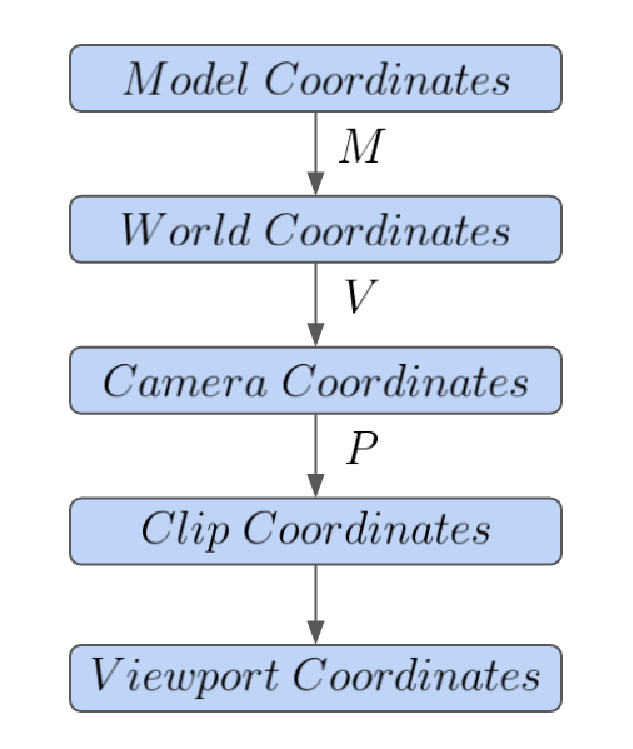
\includegraphics[width=0.3\textwidth]{images/mvp_model.pdf}
    \caption{Switching between coordinates using different transformation matrices}
    \label{fig:basic_transformations}
\end{figure}


\subsection{Disturbing Water} \label{subsec: disturbing_water}
According to business analysis user must be able to interact with the water by disturbing its surface. We assumed that the interaction will occur when the left mouse button will be pressed over the water grid. Such an action will increase water level (value on $Y$ axis) of the specific vertex. Although the concept seems straight forward there is one main obstacle - mouse works in two dimensional screen coordinates while intersection happens in three dimensional world coordinates. In a consequence, the application must adapt some procedure to translate between the two. Figure \ref{fig:screen_to_world} tries to visualize the problem of conversion.

\begin{figure}[H]
    \centering
    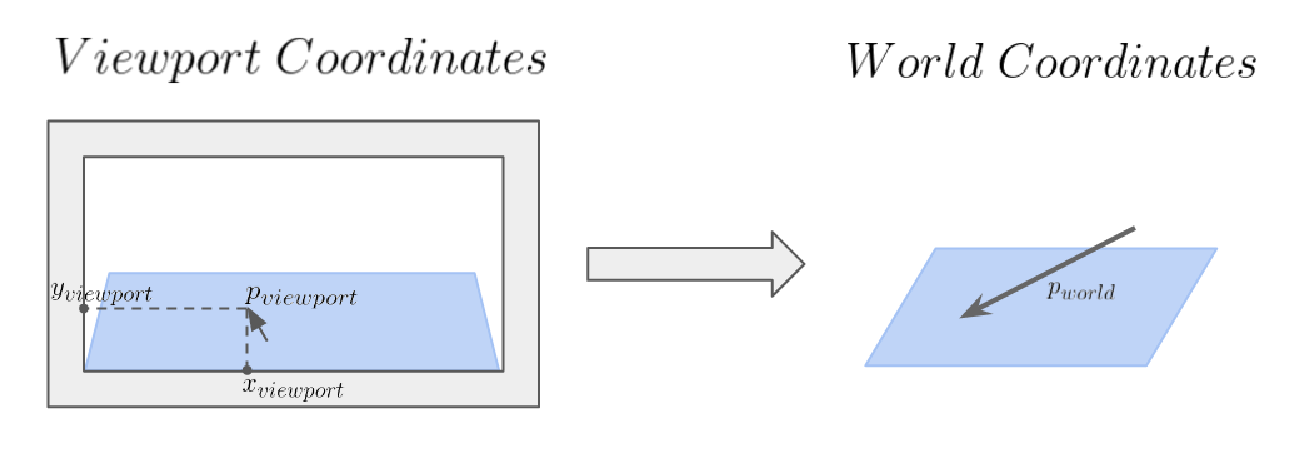
\includegraphics[width=0.7\textwidth]{images/screen_to_world.pdf}
    \caption{Conversion between two dimensional mouse input and three dimensional world coordinates is the main problem of interacting with the water. The point $p_{viewport}$ can also be thought as a pixel.}
    \label{fig:screen_to_world}
\end{figure}

To cope with the problem, the application must perform a series of transformations. To begin with, viewport coordinates of specified point $p_{viewport} \in \mathbb{R}^{2}$ must be converted to normalized device coordinates. To achieve it, following formulas should be implemented:
\begin{equation} \label{eq:to_ndc}
p_{viewport} = \begin{bmatrix}
           x_{viewport}\\
           y_{viewport}
\end{bmatrix} \; \; \; \Rightarrow \; \; \; 
p_{ndc} = \begin{bmatrix}
           \frac{2 \; \cdot \; x_{vieport}}{viewport\_width} - 1 \\
           1 - \frac{2 \; \cdot \; y_{vieport}}{viewport\_height} \\
           1
\end{bmatrix}
\end{equation}
where $p_{ndc} \in \mathbb{R}^{3}$ represents a point in normalized device coordinates; $viewport\_width$ and $viewport\_height$ defines resolution of the application's window. Equation \ref{eq:to_ndc} will place point $p_{viewport}$ in $\langle -1; 1 \rangle \times \langle -1; 1 \rangle \times \langle -1; 1 \rangle$ interval. Since by OpenGL convention, positive $Z$ axis is directed out of the screen, $p_{ndc}$'s z coordinate has been chosen to mimic the point's origin (i.e. two dimensional screen). Next, there is simple shift to clip coordinates by extending the dimensions of $p_{ndc}$ by 1 - placing it in homogeneous coordinates. The operation is performed in the following manner:
\begin{equation} \label{eq:to_clip}
p_{ndc} = \begin{bmatrix}
           x_{normalized}\\
           y_{normalized} \\
           z_{normalized}
\end{bmatrix} \; \; \; \Rightarrow \; \; \; 
p_{clip} = \begin{bmatrix}
           x_{normalized} \\
           y_{normalized} \\
           z_{normalized} \\
           1
\end{bmatrix}
\end{equation}
where $p_{clip} \in \mathbb{R}^{4}$ represents a point in clip coordinates. Freshly introduced value $1$ in the point's coordinates tells the homogeneous space that $p_{clip}$ represents a position rather than direction. Note that the point resides on near plane of the clip's cube. After that, the application must switch to camera space. To manage that, operations specified below must be applied:
\begin{equation} \label{eq:to_camera}
p_{clip} = \begin{bmatrix}
           x_{clip}\\
           y_{clip} \\
           z_{clip} \\
           w_{clip}
\end{bmatrix} \; \; \; \Rightarrow \; \; \; 
P^{-1}\begin{bmatrix}
           x_{clip}\\
           y_{clip} \\
           z_{clip} \\
           w_{clip}
\end{bmatrix} = \begin{bmatrix}
           x_{camera}\\
           y_{camera} \\
           z_{camera} \\
           w_{camera}
\end{bmatrix}  \; \; \; \Rightarrow \; \; \; 
p_{camera} = \begin{bmatrix}
           x_{camera}\\
           y_{camera} \\
           -1 \\
           0
\end{bmatrix}
\end{equation}
where $P^{-1} \in \mathbb{R}^{4 \times 4}$ represents inverse of the projection matrix and $p_{camera} \in \mathbb{R}^{4}$ is a point in camera coordinates. Last step involves changing values on $Z$ and $W$ axes. Latter one tells the space that we are dealing with a vector this time ($w = 0$), while the former orients it "into the scene" ($z=-1$). Last thing to do is conversion to world coordinates. The application will apply inverse view matrix  $V^{-1} \in \mathbb{R}^{4 \times 4}$ to a vector $p_{camera}$ and drop the 4th dimension as follows:
\begin{equation} \label{eq:to_world}
p_{camera} = \begin{bmatrix}
           x_{camera}\\
           y_{camera} \\
           z_{camera} \\
           w_{camera}
\end{bmatrix} \; \; \; \Rightarrow \; \; \; 
V^{-1}\begin{bmatrix}
           x_{camera}\\
           y_{camera} \\
           z_{camera} \\
           w_{camera}
\end{bmatrix} = \begin{bmatrix}
           x_{world}\\
           y_{world} \\
           z_{world} \\
           w_{world}
\end{bmatrix}  \; \; \; \Rightarrow \; \; \; 
p_{world} = \begin{bmatrix}
           x_{world}\\
           y_{world} \\
           z_{world}
\end{bmatrix}
\end{equation}
where $p_{world} \in \mathbb{R}^{3}$ represents desired vector in the world coordinates.

Next thing that one needs to consider is determining whether a ray intersects the grid - in the end it can miss or go parallel to the surface. It is highly recommended to refer to the Figure \ref{fig:ray_intersect}, while reading the mathematical derivation of the intersection formula. To start with, every plane can be described using a normal to its surface and a point of displacement with regard to the world coordinates origin. They are denoted as $\vec{n}$ and $p$ on Figure \ref{fig:ray_intersect}. From any point on the plane we can compute a vector by subtracting $p$ from this point. In our particular example: $\vec{p}_1 = p_1 - p$. Naturally $\vec{n}, p, p_1, \vec{p}_1  \in \mathbb{R}^3$. Since point $\vec{p_1}$ is perpendicular to the surface, following property holds:
\begin{equation} \label{eq:plane}
(p_1 - p) \circ n = 0
\end{equation}
Correspondingly, ray can be described using following parametric form:
\begin{equation} \label{eq:ray}
r + \vec{d} \cdot t = p_1
\end{equation}
where $r \in \mathbb{R}^3$ is the ray's origin and $\vec{d} \in \mathbb{R}^3$ denotes its direction. Parameter $t \in \mathbb{R}$ allows to describe any point (including the ray's origin for $t=0$) along the ray. Of course, when we are able to describe any point lying on the ray, why not to choose the one situated on the plane? To do so one should simply put equation \ref{eq:ray} into equation \ref{eq:plane}, which will produce the following:
\begin{equation}
(r + \vec{d} \cdot t - p) \circ \vec{n} = 0
\end{equation}
Solving for $t$ gives:
\begin{equation}
t = \frac{(p - r) \circ \vec{n}}{\vec{d} \circ \vec{n}}
\end{equation}

Let us stop here for a moment. One can easily observe that denominator can be equal $0$. It will happen only in case of the ray parallel to the surface and we can discriminate two possible scenarios: either the ray perfectly coincide with the plane or it is away from it. Former produces infinite number of solutions, where latter one - none of them. Nevertheless one should firstly calculate the $\vec{d} \circ \vec{n}$ to determine if further computations are needed.

\begin{figure}[H] 
    \centering
    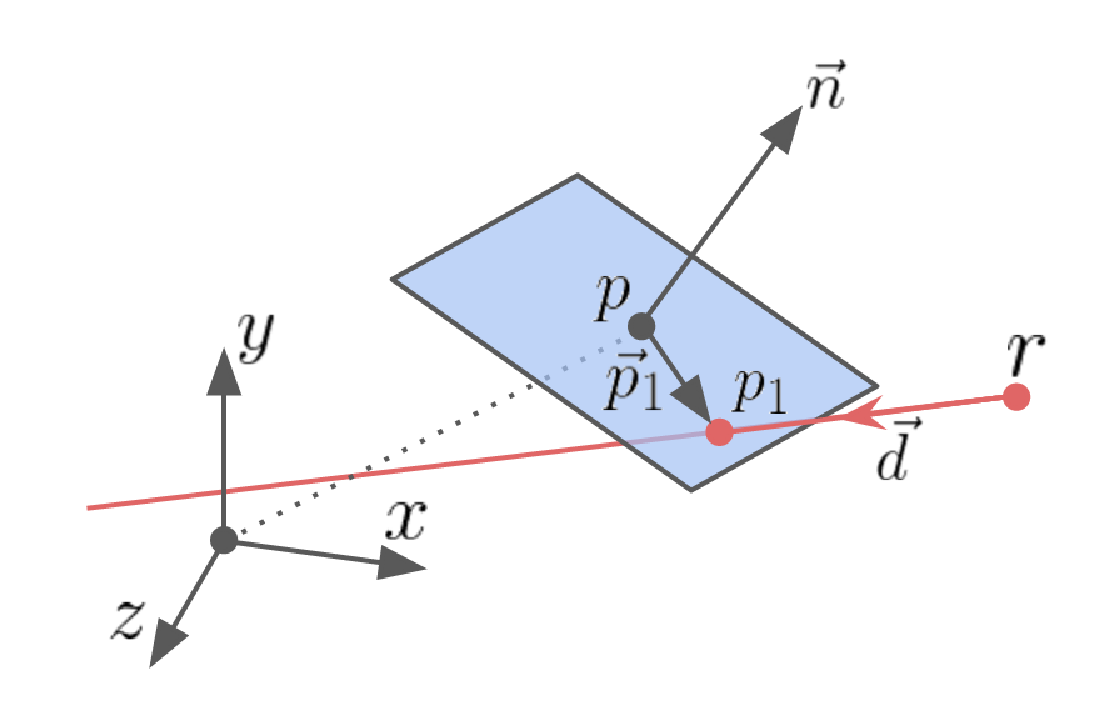
\includegraphics[width=0.4\textwidth]{images/ray_intersect.pdf}
    \caption{A ray intersecting a plane. Ray's origin is in point $r$ and its direction is described by vector $\vec{d}$. In addition, one can observe a plane with normal $\vec{n}$, shifted by $p$.}
    \label{fig:ray_intersect}
\end{figure}

But this is not all - one small thing has been left out. Above equations assume that the plane has an infinite area, which in our case is not true. To cope with that problem one need to perceive that our setup assumes that water is a plane with $ \vec{n} = \left(\begin{smallmatrix}0 \\ 1 \\0 \end{smallmatrix}\right)$ and it is entirely enclosed in $XZ$ plane. What is more, water grid belongs to the $\langle -\frac{a}{2} ; \frac{a}{2}  \rangle \times \langle -\frac{a}{2} ; \frac{a}{2}  \rangle$ interval. As a consequence when intersection point $p_1$ is found, its $x$'s and $z$'s coordinates must be enclosed by the interval . In other words:
\begin{equation}
p_1= \left(\begin{smallmatrix} x \\ y \\ z \end{smallmatrix}\right) \wedge x, z \in \langle -\frac{a}{2} ; \frac{a}{2}  \rangle  \Leftrightarrow  p_1 \in \text{water grid}
\end{equation}
where $p_1 \in \mathbb{R}^{3}$ is an intersection point and $a \in \mathbb{R}$ is grid's size (once again: we assume that the grid has square shape). 

\begin{wrapfigure}{l}{0.5\textwidth}
  \raisebox{0pt}[\dimexpr\height-0.7\baselineskip\relax]
  {
    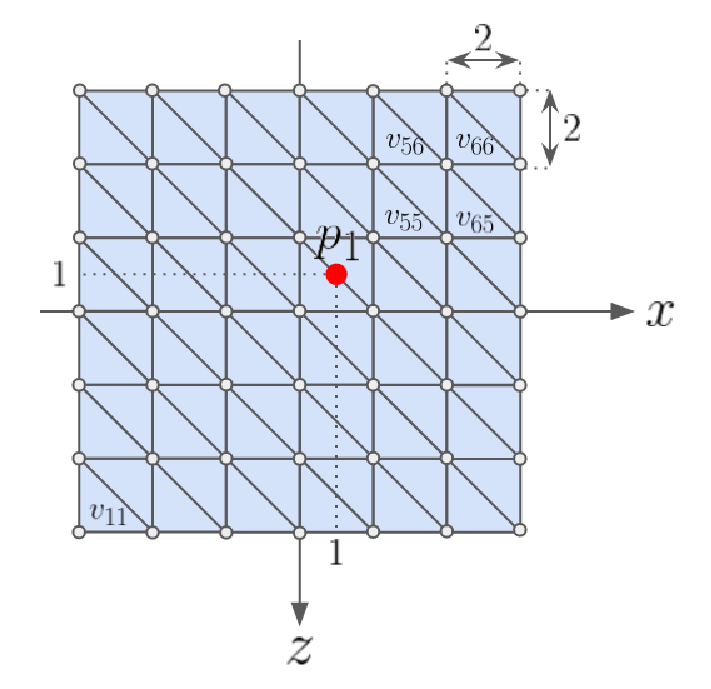
\includegraphics[width=0.75\textwidth]{images/example_quad.pdf}
  }
  \caption{Example of the intersection point on~$12 \times 12$~grid with $7$ vertices per side.}
  \label{fig:example_quad}
\end{wrapfigure}

At the end, one will be forced to find the vertex $v_{xz}$ that needs to be disturbed. Index $x$ describes vertex shift on $X$ axis and index $z$ on $Z$ axis. Please refer to Figure \ref{fig:example_quad} for a specific example. At this stage $p_1$'s $y$ value does not interest us at all, because it will be always equal to $0$ (we are playing on $XZ$ plane only and do not car about any water disturbances). Following equations cover computing appropriate indices for a vertex:
\begin{equation}
\begin{split}
x = \floor{\frac{q \cdot (p_{1x} + \frac{a}{2})}{a}} + 1\\
z = \floor{\frac{q \cdot (p_{1z} + \frac{a}{2})}{a}} + 1
\end{split}
\end{equation}
where $q \in \mathbb{Z}$ is the number of vertices per grid's side, $p_1 \in \mathbb{R}^{3}$ represents the point of intersection and $a \in \mathbb{R}$ denotes size of the grid. First, $p_{1x}$ and $p_{1z}$ are translated by $\frac{a}{2}$, which forces them to belong to the $\langle 0 ; a \rangle$ interval. To present things clearly one can move $q$ from the nominator to the denominator to create $\frac{a}{q}$ expression, which can be interpreted as a space between consecutive vertices. So by dividing $p_{1x}$ and $p_{1z}$ by $\frac{a}{q}$, one can acquire a shift in vertices from the origin on both, $X$ and $Z$ axes. Since vertices are finite entities, the formulas take the integer part of the obtained values. 

To make things a little bit more understandable let us look at an example. Figure \ref{fig:example_quad} depicts water grid with length  $a=12$ and seven vertices per side ($q=6$). As assumed it is centered at the worlds space origin. Vertices are marked as a gray circles. In addition, intersection point $p_1 = \left(\begin{smallmatrix}1 \\ 0 \\1 \end{smallmatrix}\right)$ has been marked by a red dot. Not all vertices have been marked to keep the picture readable. Their symbols follow previously assumed pattern. Using aforementioned equations one will acquire following results:
\begin{equation*}
\begin{split}
x = \floor{\frac{7 (1 + \frac{12}{2})}{12}} + 1 = \floor{\frac{49}{12}} + 1 = 4  + 1 = 5 \\
z = \floor{\frac{7 (1 + \frac{12}{2})}{12}} + 1 = \floor{\frac{49}{12}} + 1 = 4  + 1 = 5
\end{split}
\end{equation*}
hence the vertex that need to be disturbed is marked as $v_{55}$. When the vertex has been localized the application can instantly change its hight in the texture representation, which will cause the disturbance in the water surface.

Additionally, one can disturb a water with predefined function to allow modeling different kind of disruptions. The application will use following one:
\begin{equation}
f(x,y) = h + f \cdot (-x^{2} - y^{2})
\end{equation}
where $h, f \in \mathbb{R}$ are parameters that can be tweaked, $x,y \in \langle -k ; k \rangle \times \langle -k ; k \rangle $ represents a region, and $k \in \mathbb{Z}$ is called a \textit{kernel}. A kernel defines finite, discrete, square area with odd-length edge with center situated in the intersected vertex. One should note that $k$ does not involve any vertices indices and can be treated as an abstract frame around the intersection vertex. 


\subsection{Shading the Water} \label{subsection:water_shading}
To begin with, water shading is mainly based on color samples taken from surrounding skybox. In each frame, vectors incident to individual pixels are computed and based on them the program calculates reflected and refracted rays. Next, intersection points of two vectors and the skybox are estimated and used to take samples from appropriate textures.

\begin{wrapfigure}{l}{0.4\textwidth}
  \raisebox{0pt}[\dimexpr\height-0.6\baselineskip\relax]
  {
    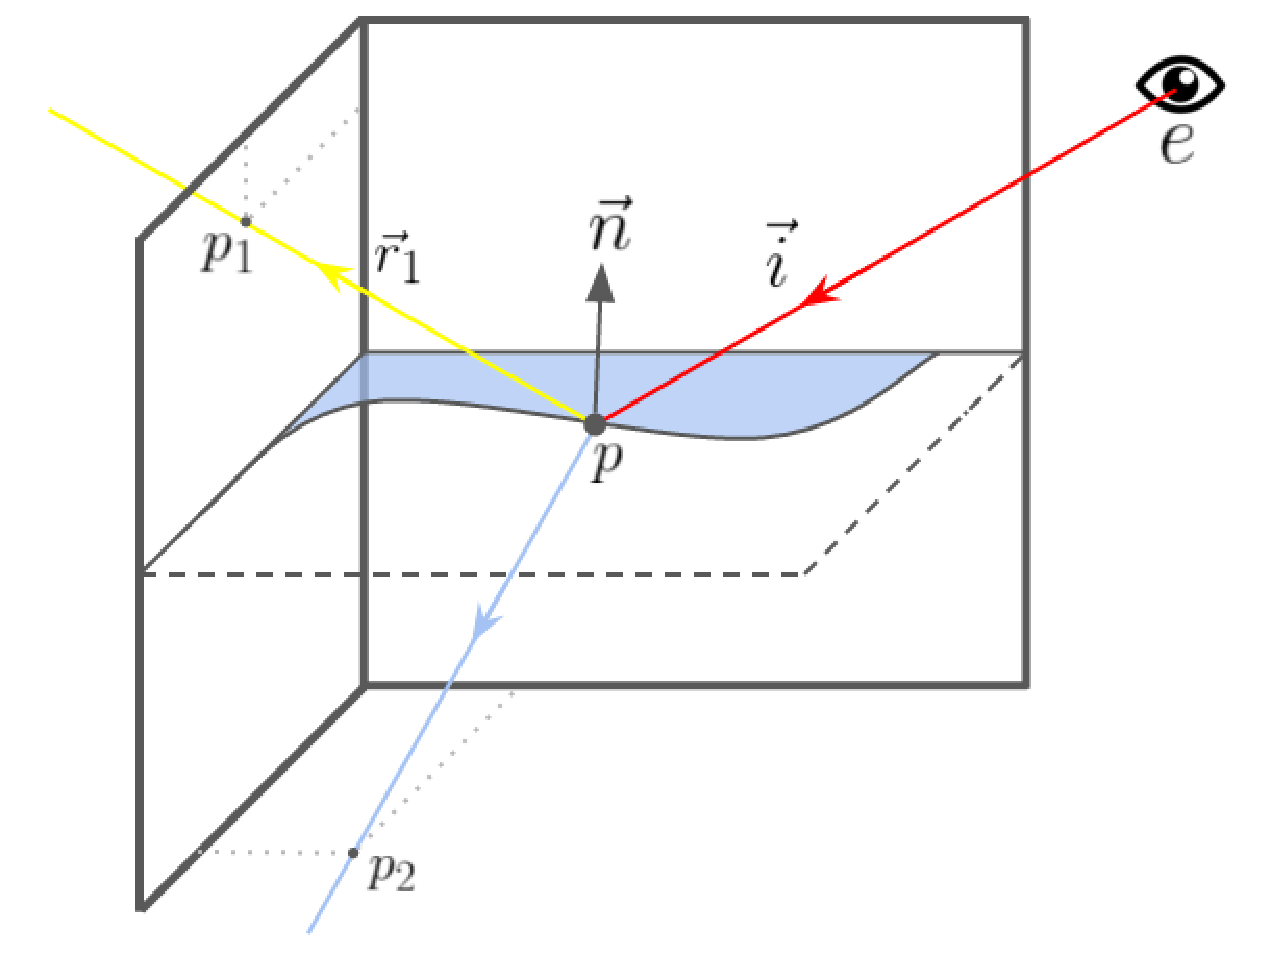
\includegraphics[width=0.9\textwidth]{images/reflection_refraction.pdf}
  }
  \caption{sdds}
  \label{fig:reflection_refraction}
\end{wrapfigure}

Figure \ref{fig:reflection_refraction} should be treated as a reference. Ray from the eye to a pixel is denoted as $\vec{i}$. Reflected and refracted rays as $\vec{r}_1$ and $\vec{r}_2$, respectively. $p_1$ is an intersection point of $\vec{r}_1$ and the skybox. Point $p_2$ has the same role but for $\vec{r}_2$. Last but not least, $\vec{n}$ represents a normal of considered pixel. Since the application knows only about two points: a pixel's position $p$ and the eye position $e$, everything else must be calculated. 

Incident ray is a result of simple subtraction:
\[
\vec{i} = p - e
\]
Reflection vector can be calcualted as follows:
\begin{equation} \label{eq:reflection_vector}
\vec{r}_1 = \vec{i} - 2 \cdot (\vec{i} \circ \vec{n}) \cdot \vec{n}
\end{equation} 
Equation \ref{eq:reflection_vector} is based on the fact that the angle between normal and an incident ray is the same as between normal and a reflected ray i.e. $\measuredangle{\vec{i}\vec{n}} = \measuredangle{\vec{i}\vec{r}_1}$. Its complete derivation is irrelevant from the paper's point of view.
Refracted ray is slightly more complicated. It can be calculated using following equation:
\begin{equation}\label{eq:refracted_vector}
\begin{split}
\vec{r}_2 = \frac{n_1}{n_2} \cdot \vec{i} - (\frac{n_1}{n_2} \cdot (\vec{n} \circ \vec{i}) + \sqrt{1 - k^{2}}) \cdot \vec{n}
\end{split}
\end{equation}
where $k = (\frac{n_1}{n_2})^{2} \cdot (1 - (\vec{n} \circ \vec{i})^{2})$, $n_1$ is a refractive index of the air and $n_2$ denotes refractive index of the water. Values of refractive indices of different materials are generally known. In case of the following paper: $n_1 = 1.0$ and $n_2 =1.333$. As before the formula's derivation has been omitted since it is quite lengthy and unimportant from the section's perspective. What is more both, Equation \ref{eq:reflection_vector} and \ref{eq:refracted_vector} are implemented as a functions in OpneGL library, so one will never encounter the formulas explicitly in the code.

Next, the intersection with the skybox must be computed. To present the algorithm, first, two dimensional case will be discussed to enable clear depicting of the vectors. At this point its extension by a 3rd dimension should be intuitive enough to just present the equations. To begin with, Figure \ref{fig:box_intersection} presents axis aligned square. It can be thought of as a Cartesian product of two intervals: $\langle x_{min} ; x_{max} \rangle$ and $\langle y_{min} ; y_{max} \rangle$. Naturally, $ x_{min}, x_{max}, y_{min}, y_{max} \in \mathbb{R}$. A ray, with its origin in point $r \in \mathbb{R}^{3}$, has been shot in direction $\vec{d} \in \mathbb{R}^{3}$. By splitting $r$ to its separate components ($r_x$ on $X$ axis and $r_y$ on $Y$ axis), following equations can be defined:
\begin{equation*}
\begin{split}
r_x + t_{min_{x}} \cdot \vec{d}_x = x_{min} \\
r_y + t_{min_{y}} \cdot \vec{d} = y_{min}  \\
\end{split}
\end{equation*}
where $t_{min_{x}}$, $t_{min_{y}} $ $\in \mathbb{R}$. Solving for  $t_{min}$'s gives: 
\begin{equation*}
\begin{split}
t_{min_{x}} = \frac{(x_{min} - r_x)}{\vec{d}_x}\\
t_{min_{y}} = \frac{(y_{min} - r_y)}{\vec{d}_y}
\end{split}
\end{equation*}
Similarly, one can compute $t_{max_{x}}$ and $t_{max_{y}}$:
\begin{equation*} 
\begin{split}
t_{max_{x}} = \frac{(x_{max} - r_x)}{\vec{d}_x}\\
t_{max_{y}} = \frac{(y_{max} - r_y)}{\vec{d}_y}
\end{split}
\end{equation*}
where $t_{max_{x}}$, $t_{max_{y}} $ $\in \mathbb{R}$. As one can notice all $t$'s are in the $\langle 0 ; 1 \rangle$ interval. It is because $t_{max}$'s represent a fraction of $\vec{d}$ to $p_1$. Correspondingly, $t_{min}$'s constitute a fraction of $\vec{d}$ to $p_2$. Finally, one can obtain $t_{min}$ and $t_{max}$:
\begin{equation*}
\begin{split}
t_{min} = \max (t_{min_x} , t_{min_y} )\\
t_{max} = \min (t_{max_x} , t_{max_y})
\end{split}
\end{equation*}
which results in explicit solutions:
\begin{equation}\label{eq:box_intersection}
\begin{split}
p_1 = r + t_{min} \cdot \vec{d} \\
p_2 = r + t_{max} \cdot \vec{d} 
\end{split}
\end{equation}

\begin{figure}[H] 
    \centering
    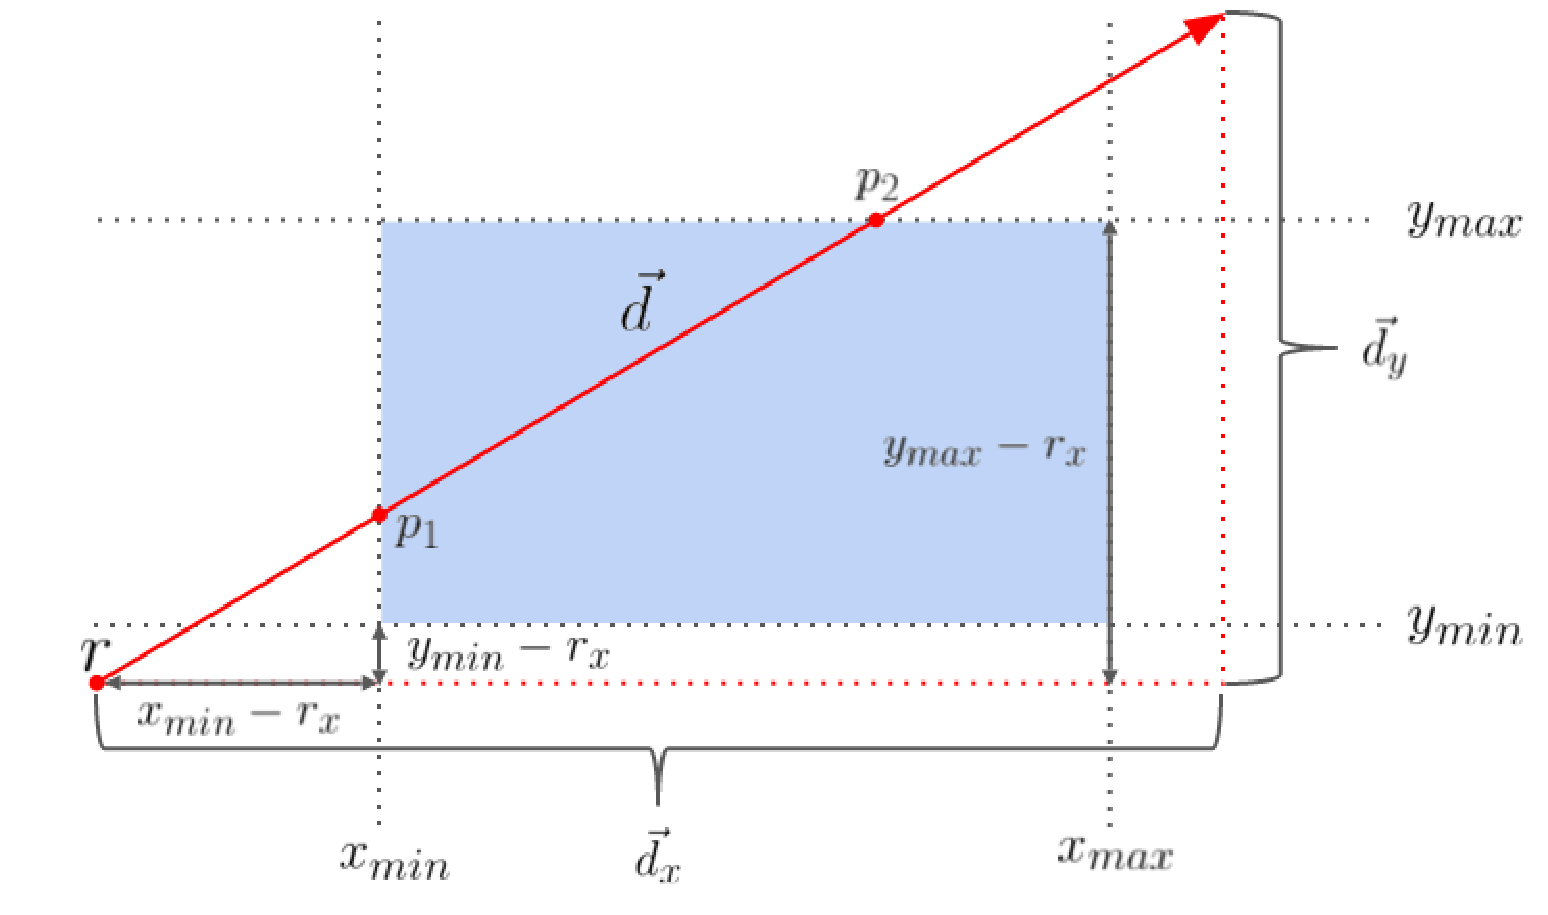
\includegraphics[width=0.5\textwidth]{images/box_intersection.pdf}
    \caption{A ray of origin $r$ and direction $\vec{d}$ intersects a box enclosed by $\langle x_{min} ; x_{max} \rangle \times \langle y_{min} ; y_{max} \rangle$ interval.}
    \label{fig:box_intersection}
\end{figure}

Of course application requires three dimensional approach. Simple algorithm's extension, by adding additional coordinate z will fix that issue. Since steps are almost similar, only formulas related to the new coordinate are presented:
\begin{align*}
t_{min_{z}} = \frac{(z_{min} - r_z)}{\vec{d}_z} & \; \; \; t_{min} = \max (\max (t_{min_x} , t_{min_y}), t_{min_z} )\\
t_{max_{z}} = \frac{(z_{max} - r_z)}{\vec{d}_z} & \; \; \; t_{min} = \min (\min (t_{max_x} , t_{max_y}), t_{max_z} )
\end{align*}
Once again, Equation \ref{eq:box_intersection} can be used to find the solution. 

At this stage the application is in poses of two intersection points $p_1$ and $p_2$. With usage of OpenGL's internal functions, former one is translated to color $c_1$ and the latter one to $c_2$. Transformation simply takes the points and samples respective colors from the skybox's textures. Now, the application must mix the colors with appropriate ratio . For example if the ratio equals $0.5$, $50\%$ of resulting color will come from $c_1$ and the other half from $c_2$. But with ratio $0.7$, $c_1$ will constitute $70\%$ of the output color, while $c_2$ only $30 \%$. Ratio can be thought of as an impact that a partial colors have on the output color. Using Schlick's approximation, ratio $s$ can be calculated as follows:
\begin{equation} \label{eq:schlick}
s = s_0 + (1 - s_0) \cdot (1 - (\vec{n} \circ -\vec{i}))^{5}
\end{equation}
where $s_0 = (\frac{n_1 - n_2}{n_1 + n_2})^{2}$, $n_1 = 1.0$ is a refractive index of the air and $n_2 = 1.333$ denotes refractive index of the water. One should note that $\vec{i}$ has been negated to represent vector directed to the eye. Equation \ref{eq:schlick} approximates the Frasnel Factor and is widely used in computer graphics. To finish with, the application will call OpenGL's \texttt{mix} function as follows: \texttt{mix($c_1$,$c_2$,$s$)}, to produce the final color of considered pixel.

\subsection{Water Simulation} \label{subsec:water_simulation}
Following section will take a top-down approach. First, general method and data structures used for water waves computations will be presented. One will come to know how off-screen rendering methods are used to process high amount of data in a parallelized manner. Next, the numerical algorithm, along with its mathematical derivation, will be introduced. Note that the section operates on OpenGL's data structures such as textures or frame buffer objects. Although they are described in a very general matter, one is suggested to refer to other source in case of any misunderstandings or lack of knowledge. This will assure full understand of the explained procedures

\subsubsection{Updating The Surface}
Each application's frame should perform consecutive step of the water simulation process. It is rather obvious that when no disturbance in water surfaces has occurred, no water displacement will take place. On the other hand, when some external factor has roiled the fluid surface, the program should instantly react and simulate successive steps of the simulation. As a consequence, per-frame analyze of the water surface representation is necessary. 

As mentioned in section \ref{subsec:scene_setup}, water is represented by $n \times n$ grid, where $n$ defines number of vertices per side. Originally, water is assumed to be flat (i.e. each vertex of the grid has its $y$ value set to $0$) and any displacement during water simulation will affect only values on $Y$ axis. As a result, $x$ and $z$ coordinates become redundant (in terms of the simulation process) and only height of each vertex is considered. What is more, both of the numerical solutions, described in next sections, require some information from previous steps of the simulation, which need to be stored.

\begin{figure}[H]
    \centering
    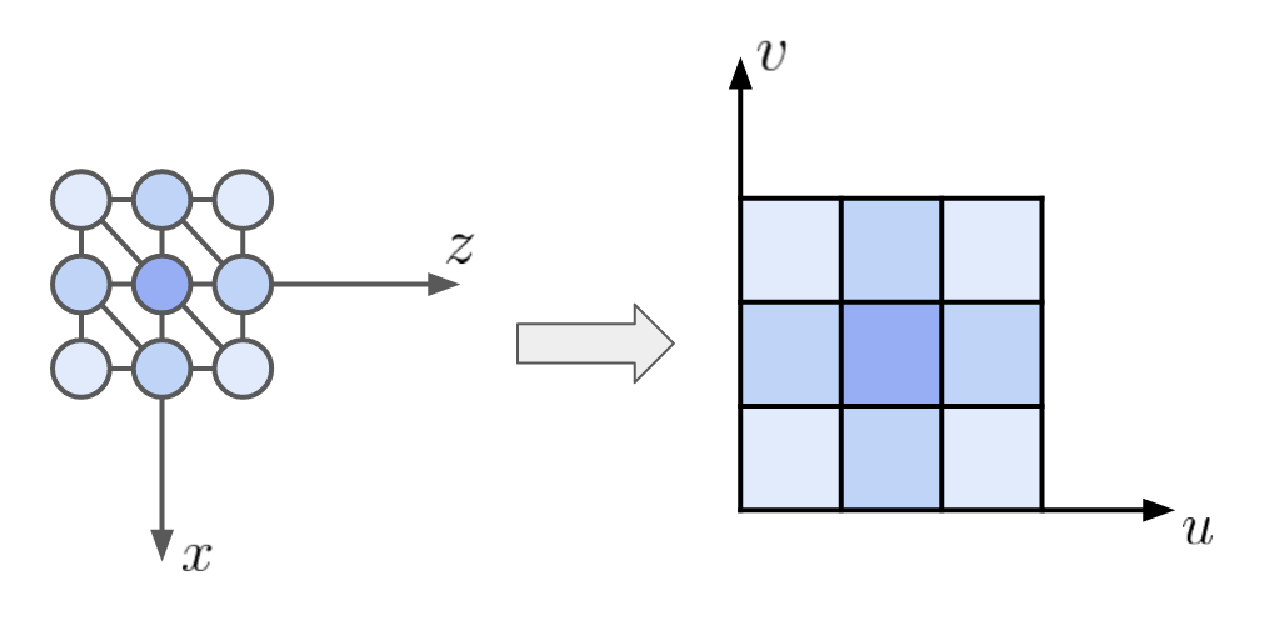
\includegraphics[width=0.6\textwidth]{images/grid_to_tex.pdf}
    \caption{Image depicts concept of transition from 3D grid's vertices to the 2D texture. From the left one can observe sample of water grid, projected on $XZ$-plane. Its vertices has benn marked as a circles with different colors according to their values on Y-axis. At the right hand side, resulting 2D texture is shown. Heights of vertices are stored in the blue channel.}
    \label{fig:grid_to_tex}
\end{figure}

To fulfill all the demands, we have used $n \times n$, RGBA texture object, later referred to as water displacement texture. Its pixels are capable of storing floating value in each channel, which gives great flexibility in terms of information saving. It is essential to realize that individual pixel corresponds to some particular vertex of the grid. As an example, let us use figure \ref{fig:grid_to_tex} - rather simplified version of the problem. Starting from the left hand side, there is its the water grid projection on $XZ$-plane, where each circle represents a vertex. Particular color corresponds to the current height of a vertex (its value on $Y$ axis). 3 different heights (in saturation of blue) are presented. Darker a color, greater a $y$ value. On the right hand side, image shows the 2 dimensional texture. Its blue channel has been used to store the grid's heights. In the result, pixels that hold greater heights are more bluish than those corresponding to the lower ones. One should remember, that following picture is just a general example of the idea and should be not treated as its specific implementation.

Next we will tackle the problem of updating water displacement texture. As for now, precise equations will be omitted in favor of a general algorithm's flow. To start with, we assume two water displacement textures - $TEX_0$ and $TEX_1$. Both of them should contain the same data and be of the same dimensions. Alongside, two frame buffer objects are created: $FBO_0$ and $FBO_1$. Relation between textures and frame buffers is as follows:

\begin{itemize}
\item $FBO_0$'s color attachment is $TEX_0$.
\item $FBO_1$'s color attachment is $TEX_1$.
\end{itemize}

In other words, $FBO_0$ and $FBO_1$ will render to $TEX_0$ and $TEX_1$, respectively. They will be alternatively called output textures (e.g.  $TEX_1$ is the output texture of $FBO_1$ etc.). What is more, both frame buffer objects will execute the same shader program. The program will accept input texture (binded one) and based on information stored in its pixels, will compute the output texture. Two off-screen rendering passes are assumed, first one performed by $FBO_1$ and second by $FBO_0$. We present figure \ref{fig:fbo_algo}, which will be analyzed step by step to better grasp the idea.

To start with, $TEX_0$ is binded. Next, $FBO_1$ will read the information from the binded texture, use them to compute heights for the next simulation's step and save the results in $TEX_1$. Then we bind $TEX_1$ (with fresh data) and perform computations in $FBO_0$. This on the other hand, will result in saving next step of the simulation in the $TEX_0$, which is binded at the end. Water grid reads $TEX_1$'s values and updates its vertices heights.

As one can notice, two simulation steps are computed between updating the water grid. Although it seems like some information can be lost, in fact no observable degrading has been caught in early tests. Obviously animation will speed up two times, but it constitutes rather a minor problem. On the other hand, an alternative solution involves one off-screen pass and a process of tracking, which of the textures was binded last time and swaping them. What is more, similar approach must be taken during disturbing the water - which texture should be alternate if intersection occured? As a consequence, we decided to implement former, clean method, which can clearly contribute to the code transparency.



\begin{figure}[H]
    \centering
    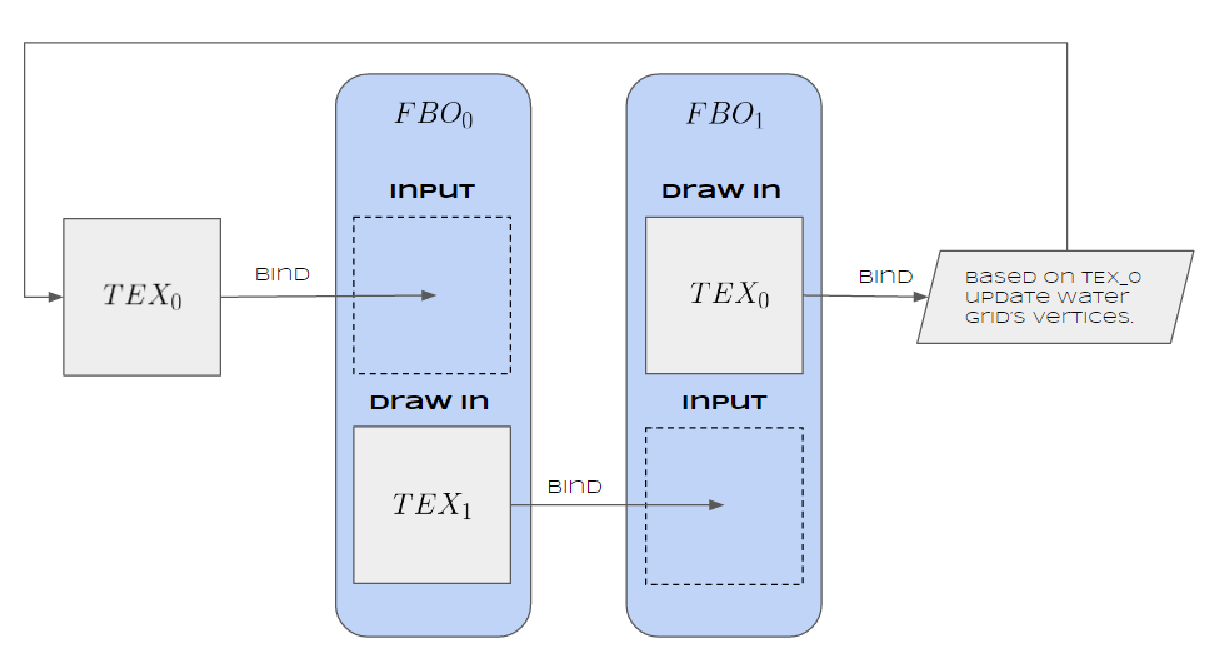
\includegraphics[width=0.8\textwidth]{images/fbo_tex.pdf}
    \caption{Updating water displacement texture algorithm. }
    \label{fig:fbo_algo}
\end{figure}


\subsubsection{Finite Difference Method}
Following section covers all aspects of the water simulation's mathematics. Although implemented equations are widely known, the paper additionally copes with deriving them using presented mathematical tools. Such approach gives the reader more insight and intuition about the topic. 

\begin{wrapfigure}{l}{0.4\textwidth}
  \raisebox{0pt}[\dimexpr\height-0.6\baselineskip\relax]
  {
    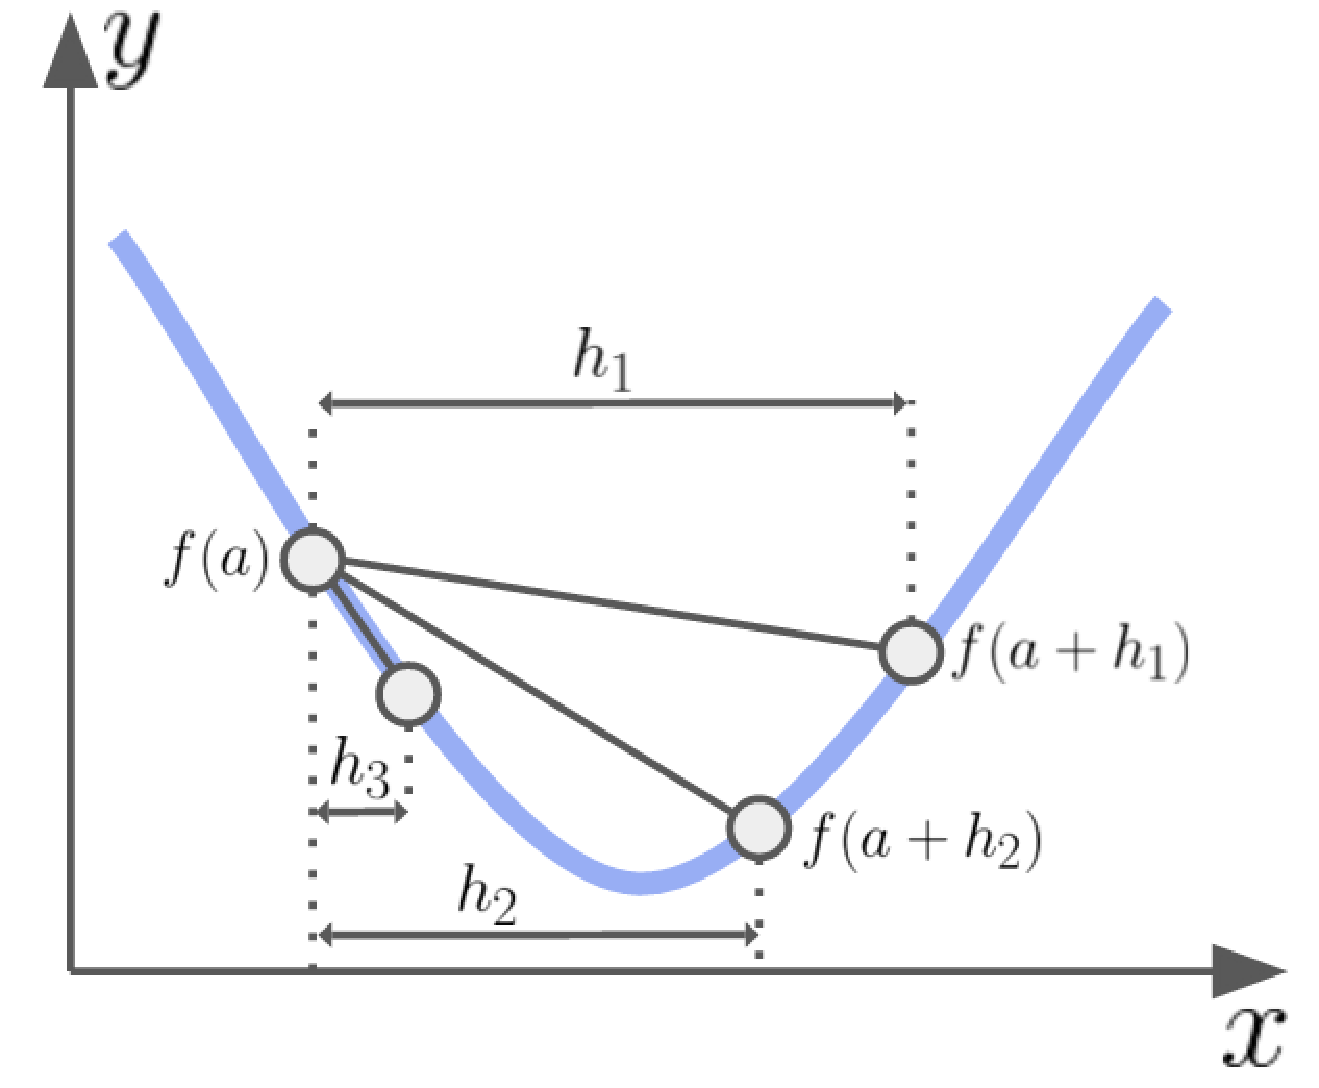
\includegraphics[width=0.8\textwidth]{images/derivative.pdf}
  }
  \caption{Example of 3 consecutive values for $h$ variable in the derivate formula (Equation \ref{eq:derivative_formula}).}
  \label{fig:derivative}
\end{wrapfigure}

Finite difference method constitutes the basic block of the simulation. It solves differential equations by approximating their derivatives. One should firstly look at the elemental derivative formula:
\begin{equation} \label{eq:derivative_formula}
f'(a) = \lim_{h \rightarrow 0} \frac{f(a+h) - f(a)}{h}
\end{equation}
where $a, h \in \mathbb{R}$ and $f: \mathbb{R} \rightarrow \mathbb{R}$. Figure \ref{fig:derivative} may be used as a reference. The picture presents consecutive shrinking of $h$ variable, hence concerns $\lim$ operation. The biggest problem with representing derivatives in the computer is that the machines cannot store abstract objects like infinitesimal values. Finite difference method confront that slight inconvenience and assumes fixed space length between consecutive steps. It basically means that $h$ value will have permanent length. In a result following approximation can be presumed:
\begin{equation} \label{eq:difference}
f'(a) \approx \frac{f(a+h) - f(a)}{h} = \frac{\Delta f}{\Delta x}
\end{equation}
Equation \ref{eq:difference} discretizes function $f$ on a grid. Result can be seen on the example presented on Figure \ref{fig:finite_diff}. Three points along with corresponding function $f: \mathbb{R} \rightarrow \mathbb{R}$ values has been marked. Length of the space between points is represented by $\Delta x \in \mathbb{R}$ and can be obtained by simple point-from-point subtraction.

\begin{figure}[H]
    \centering
    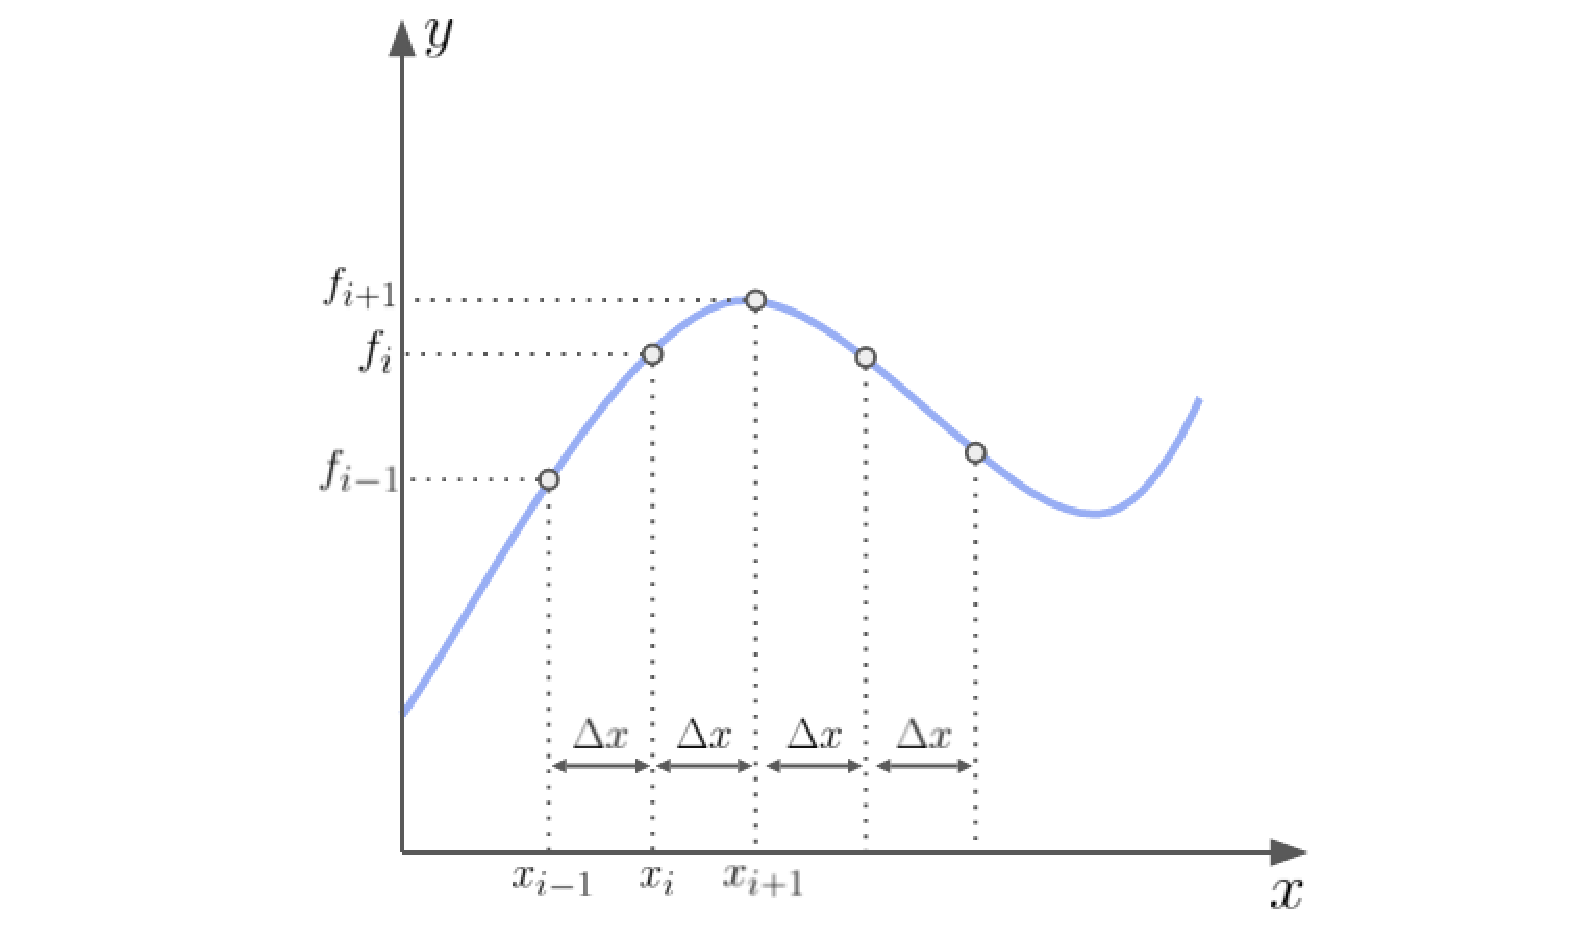
\includegraphics[width=0.6\textwidth]{images/finite_diff.pdf}
    \caption{Example of how finite difference method discretizes a function.}
    \label{fig:finite_diff}
\end{figure}

There exist three types of scheme regarding finite difference method:
\begin{itemize}
\item \textbf{Forward Difference}

Rate of change of function $f$, denoted as $\Delta f$ (Equation \ref{eq:difference}) is computed for the considered point $x_i$ and the forward step $x_{i+1}$. In other words $\Delta f = f_{i+1} - f_i$. Following assumption allows one to assume following approximation of a differential of function $f$ in point $x_i$:


\begin{equation} \label{eq:forward_diff}
f'(x_i) = \frac{df(x_i)}{dx} \approx \frac{f(x_i + \Delta x) - f(x_i)}{\Delta x} = \frac{f_{i+1} - f_i}{\Delta x}
\end{equation}

Naturally, the equation can be extended to an arbitrary order. Following formula constitutes an example of the derivation of 2nd order finite forward difference, based on Equation \ref{eq:derivative_formula} and \ref{eq:forward_diff}:
\begin{equation*}
f''(x_i) = \frac{d^2 f(x_i)}{dx^2}=\frac{d}{dx} (\frac{d \; f(x_i)}{dx}) = \frac{d}{dx} (\lim_{\Delta x \rightarrow 0}\frac{f(x_i + \Delta x) - f(x_i)}{\Delta x}) =  \lim_{\Delta x \rightarrow 0}\frac{ \frac{d}{dx} f(x_i + \Delta x) - \frac{d}{dx} f(x_i)}{\Delta x} 
\end{equation*}
Dropping the $lim$ operation, as in Equation \ref{eq:difference}, results in:
\begin{equation*}
f''(x_i) \approx \frac{ \frac{f(x_i + 2 \Delta x) - f(x_i + \Delta x)}{\Delta x}  - \frac{f(x_i + \Delta x) - f(x_i)}{\Delta x}}{\Delta x} 
\end{equation*}
which is a little bit to lengthy and can be easily simplified by merging the denominators:
\begin{equation*}
f''(x_i) \approx \frac{f(x_i + 2\Delta x) - 2 f(x_i + \Delta x) + f(x_i)}{\Delta x ^ 2} 
\end{equation*}
Furthermore, applying notation from Figure \ref{fig:finite_diff}, one will obtain:
\begin{equation} \label{eq:forward_2nd}
f''(x_i) \approx \frac{f_{i+2} - 2 f_{i+1} + f_{i}}{\Delta x ^ 2}
\end{equation}
\item \textbf{Backward finite difference}

This time, $\Delta f$ will be computed for the point $x_i$ and $x_{i-1}$, namely:
\begin{equation} \label{eq:backward_diff}
f'(x_i) = \frac{df(x_i)}{dx} \approx \frac{f(x_i) -f(x_i + \Delta x)}{\Delta x} = \frac{f_i - f_{i-1}}{\Delta x}
\end{equation}
Corresponding to Equation \ref{eq:forward_2nd}, 2nd order backward finite distance looks as follows:
\begin{equation*}
f''(x_i) \approx \frac{f_{i+2} - 2 f_{i-1} + f_{i-2}}{\Delta x ^ 2}
\end{equation*}

\item \textbf{Central finite difference}

The approach is slightly different. It presumes that the rate of change of function $f$ will be calculated using step at point $x_{i-1}$, and the forward one, at $x_{i+1}$. As a result, one acquires:
\begin{equation} \label{eq:central_bigstep}
f'(x_i) = \frac{df(x_i)}{dx} \approx \frac{f(x_i + \Delta x) -f(x_i - \Delta x)}{\Delta x + \Delta x} = \frac{f_{i+1} - f_{i-1}}{2\Delta x}
\end{equation}

\begin{figure}[H]
    \centering
    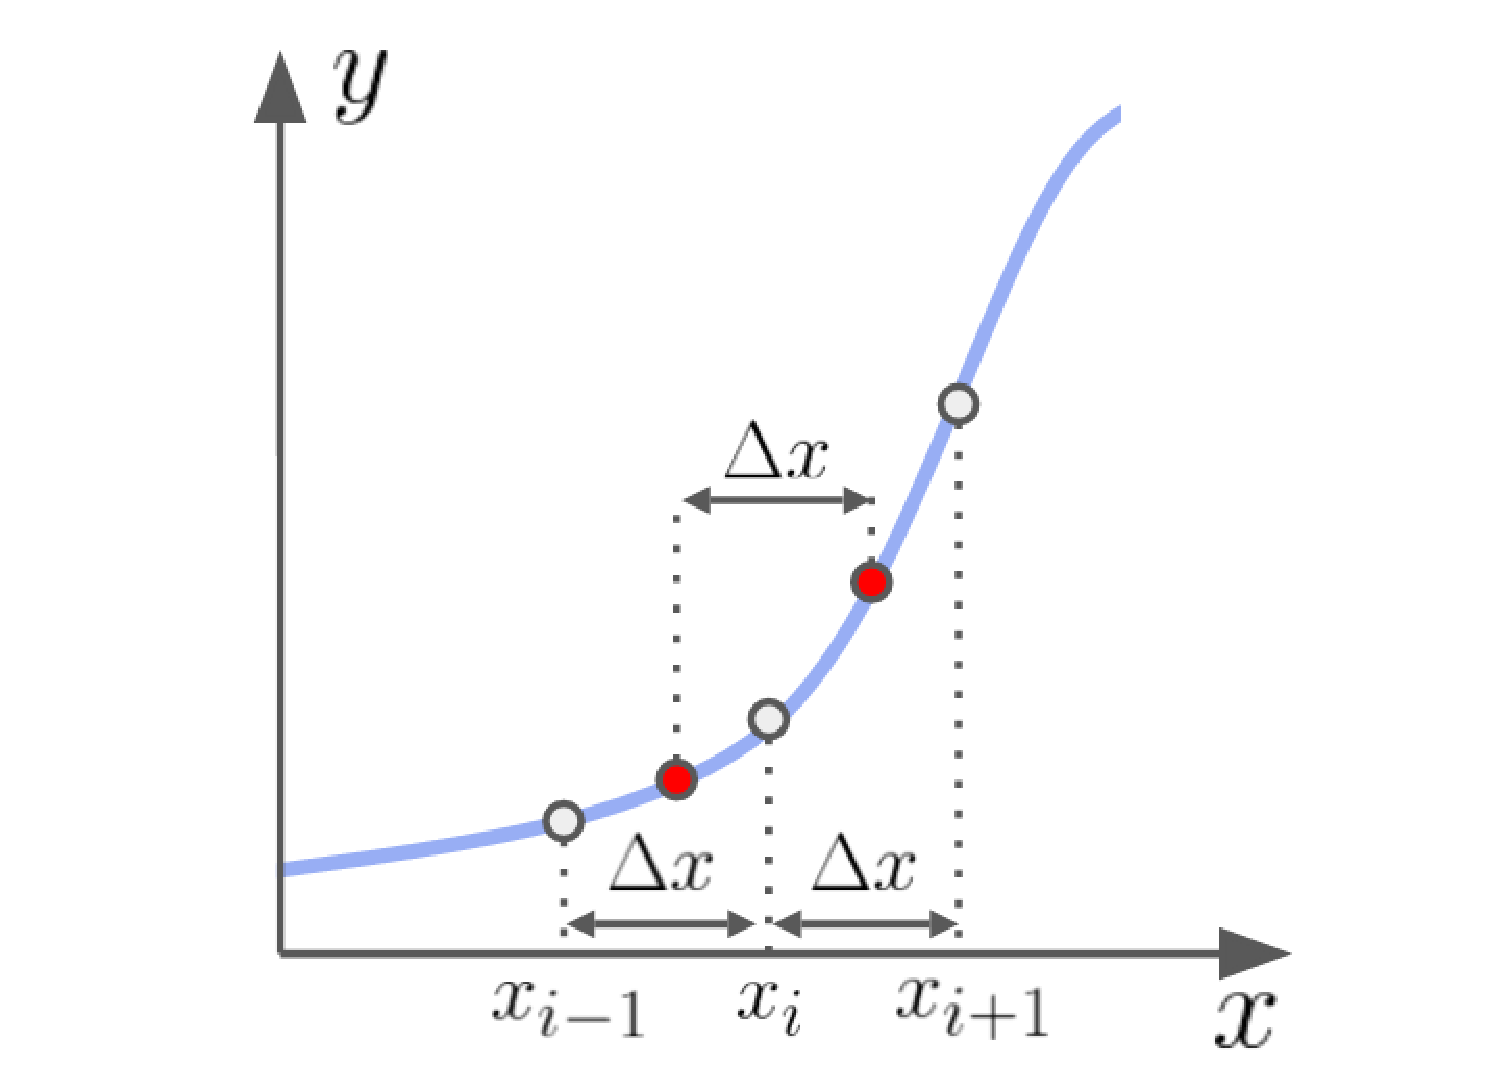
\includegraphics[width=0.35\textwidth]{images/central_diff.pdf}
    \caption{Central difference example. Red dots symbolizes the 'half-points', which increases the formula's accuracy.}
    \label{fig:central_diff}
\end{figure}

Unfortunately, Equation \ref{eq:central_bigstep} involves rather big step (with respect to accuracy) equal to $2\Delta x$. To cope with that issue one can reduce the step size in both, forward and backward step. Figure \ref{fig:central_diff} resemble an example of hypothetical situation when the central difference is calculated. Its red dots represent the 'middle-steps'. As a result, following equation can be composed:
\begin{equation*}
f'(x_i) \approx \frac{f(x_i + \frac{1}{2}\Delta x) -f(x_i - \frac{1}{2}\Delta x)}{\frac{1}{2}\Delta x + \frac{1}{2}\Delta x}
\end{equation*}
Via applying a shortcut notation one will get:
\begin{equation*}
f'(x_i) \approx \frac{  f_{i + \frac{1}{2}} - f_{i - \frac{1}{2}} }{\Delta x}
\end{equation*}

Once again, 2nd order scheme must be presented:
\begin{equation*}
f''(x_i) \approx \frac{f_{i+1} - 2 f_{i} + f_{i-1}}{\Delta x ^ 2}
\end{equation*}
\end{itemize}

Formula for 2nd order central difference will be indispensable in terms of numerical approximation. It will estimate partial derivatives and allow computer interpretation of the equations. Although presented ideas concern two dimensional function $f$, extension to higher order is rather straight forward. Let us assume that $g(x,y): \mathbb{R}^{3} \rightarrow \mathbb{R}$, then using central difference method one can obtain:
\begin{equation*}
\frac{\partial^2g(x_i,y_j,z_t)}{\partial x^2} \approx \frac{g_{i+1 , j, t} - 2 g_{i , j, t} + g_{i-1 , j, t}}{\Delta x ^ 2}
\end{equation*}
where $g_{i+1 , j, t}$, $g_{i-1 , j, t}$ and $g_{i , j, t}$ represent function $g$ shifted by $\Delta x$, $-\Delta x$ and $0$ on $x$ axis respectively.

\subsubsection{Shallow Water Equation}

Implemented equation is based solely on \cite{gomez} and will be presented here with some minor extensions. Method is a straight forward approach with usage of generally known formulas. Derivation will start from basic wave equation:
\begin{equation}
\frac{\partial^2u}{\partial t^2} = c^{2} \cdot (\frac{\partial^2u}{\partial x^2})
\end{equation}
where $c$ is the speed of wave propagation and $u(x,t)$ simulates mechanical displacement of a string. Since the equation is one space dimensional - should be extended. Membrane equation constitutes a natural extension:
\begin{equation} \label{eq:membran_eq}
\frac{\partial^2u}{\partial t^2} = c^{2} \cdot (\frac{\partial^2u}{\partial x^2} + \frac{\partial^2u}{\partial y^2}) \; \; \texttt{for} \; \; (x,y) \in \kappa
\end{equation}
where $\kappa$ is a square of side $a$ centered at the origin and  $u(x,y,t)$ is the height of a membrane at point $(x,y) \in \kappa$ at any time $t$. In our case $u = 0$ on $\partial \kappa$. 

Applying second central difference scheme to all derivatives from Equation \ref{eq:membran_eq} separately, i.e $\frac {\partial{^2u}}{\partial t^2}$, $\frac{\partial^2u}{\partial x^2}$, $\frac{\partial^2u}{\partial y^2}$, results in:
\begin{equation*}
\frac{u_{i , j, t+1} - 2 u_{i , j, t} + g_{i , j, t-1}}{\Delta t ^ 2} = c^2 \cdot (\frac{u_{i+1 , j, t} - 2 u_{i , j, t} + u_{i-1 , j, t}}{\Delta x ^ 2} + \frac{u_{i , j+1, t} - 2 u_{i , j, t} + u_{i , j-1, t}}{\Delta y ^ 2})
\end{equation*}
Assuming that $\Delta x^2 = \Delta y^2 = h^2$ and with small algebraic operation one can acquire:
\begin{equation} \label{eq:shallow_water_basic}
u_{i , j, t+1} = (\frac{c \cdot \Delta t}{h})^{2} \cdot (u_{i+1 , j, t} + u_{i-1 , j, t} - 4 u_{i , j, t} + u_{i , j-1, t} + u_{i , j+1, t}) +2 \cdot u_{i,j,t} + u_{i,j,t-1}
\end{equation}
which looks just scary. Nevertheless, analyzing the equation a little bit further reveals its simplicity. To start with, $u_{i , j, t+1}$ is a new height of point $(x_i, y_i)$, hence something that one wants to acquire in each frame. Trailing $u_{i,j,t-1}$ represents value of the point in previous pass ($t-1$), while $u_{i+1 , j, t}$, $u_{i-1 , j, t}$, $u_{i , j-1, t}$ and $ u_{i , j+1, t}$ 
are current values of four neighbors of point $(x_i, y_j)$. Obviously, $u_{i , j, t}$ denotes present value of the considered point and $\Delta t$, $h$ are just parameters.

As \cite{gomez} suggest, for the equation to be stable: $(\frac{c \cdot \Delta t}{h})^{2} \leq \frac{1}{2}$. Following constants provide correct work of the algorithm: $c = 1$, $h = \frac{2}{n-1}$ $\Delta t = \frac{1}{n}$, where $n$ denotes number of vertices per side in the water's grid. In addition, multiplying $u_{i , j, t+1}$ via $d_{i,j} = 0.95 \cdot \min(1,\frac{l}{0.2})$, where $l$ is a maximum distance from the water's grid border from a particular point, results in waves damping.

\subsubsection{Waves}
In order to make the scene more realistic, random waves function has been adapted. It is based on widely known \textit{Seascape} shader by Alexander Alekseev \cite{shader_seascape}. In particular, the shader's randomizer is used to transform the grid. Since it is just an extra feature, rather than the project's demand, mathematics behind the function will be treated as beyond the scope of the paper and will be omitted. Note that both - manual disturbance of the surface and random wave function are added in each frame to create a final heightfield of the grid.

\subsection{Ship Simulation} \label{subsec:ship_simulation}
First of all, one needs to realize that the ship's movement will be simulated with
usage of a mathematical/numerical model. A model itself is not ideal and many types of compromises must be made. Among all of them two seems most relevant: 
\begin{itemize}
\item only water will have influence on the ship (not another way around)
\item ship will be treated as a rigid body approximated using grid of cubes. 
\end{itemize} 
Furthermore, all computations regarding rigid body will be held by PhysX library. The library's API provides a means for defining an object composed of primitive shapes. For the project needs, one will have to use cubes to approximate the ship. Naturally, a box's properties like position, mass or density are easily set.
Having that, the library implements a way to add a force in a point. The functionality will be used to apply buoyancy force. Fulfilling ale aforementioned requirements will allow PhysX to estimate transformations of the ship's body in each frame. All intermediate aspects like, moment of inertia tensors or torque are handled by the library.

\subsubsection{The Simulation Algorithm}
Hull is unfortunately irregular enough to prevent analytical solution of buoyancy center. To cope with that problem, finite volume method has been adapted. Step that needs to be done before the application lunch is to approximate the ship's hull with a multiple cubes. Cubes must be of same size and they are assumed to consume 1$m^3$. We will call it computational grid and a single cube will be addressed as a cell. Naturally, smaller the cells, more the accuracy. The grid will be predefined in a file and loaded during the launch. In fact, parallely there will exist two grids - one in PhysX and second in the program. The former one is obviously required to perform computations, while the latter is present due to debugging purposes. Although one mimics another, PhysX objects need to be additionally supplied with a list of masses and densities per cell. The specifications will be chosen based on how well they simulate the ship's responses. Subfigure \ref{fig:ship_algo_1} presents a ship with its computational grid and surrounding water level in two dimensional projection. One can observe how the grid roughly approximates the hall.   

Following list contains the ship's simulation steps that need to be done per frame:
\begin{enumerate}
\item Estimate immersed part of computational grid (Figure \ref{fig:ship_algo_2})
\item Compute buoyancy center $b$ (Figure \ref{fig:ship_algo_3})
\item Calculate buoyancy force $f_b$ (Figure \ref{fig:ship_algo_4})
\item Supply PhysX with $f_b$ at point $b$ (Figure \ref{fig:ship_algo_5})
\item Receive from PhysX transformations for a next time step and apply them to the ship's model and its grid (Figure \ref{fig:ship_algo_6})
\end{enumerate}
Following subsections will cope with each task separately, providing as much details as possible. What is more, subsection \ref{subsub:physX} presents sketch of computations that are done behind the scenes by PhysX library.

\begin{figure}[htb]
    \centering % <-- added
\begin{subfigure}{0.25\textwidth}
  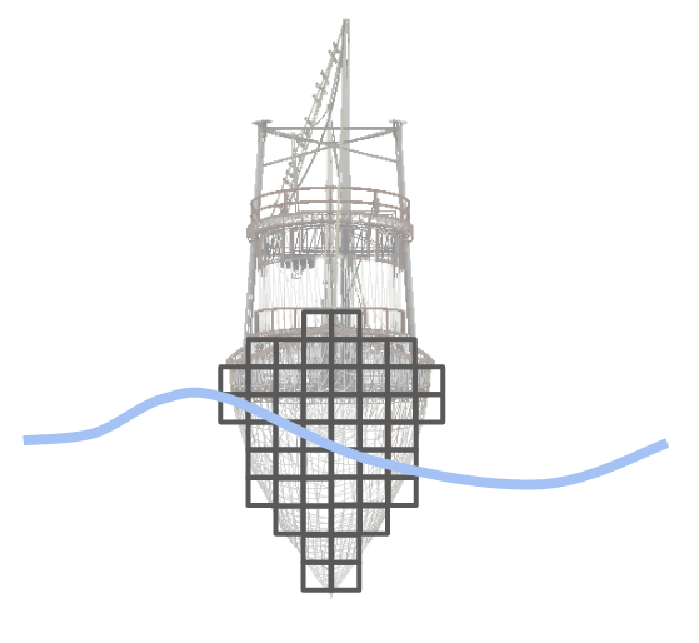
\includegraphics[width=\linewidth]{images/ship_algo_1.pdf}
  \caption{Computational grid and the ship's model in two dimensional projection.}
  \label{fig:ship_algo_1}
\end{subfigure}\hfil % <-- added
\begin{subfigure}{0.25\textwidth}
  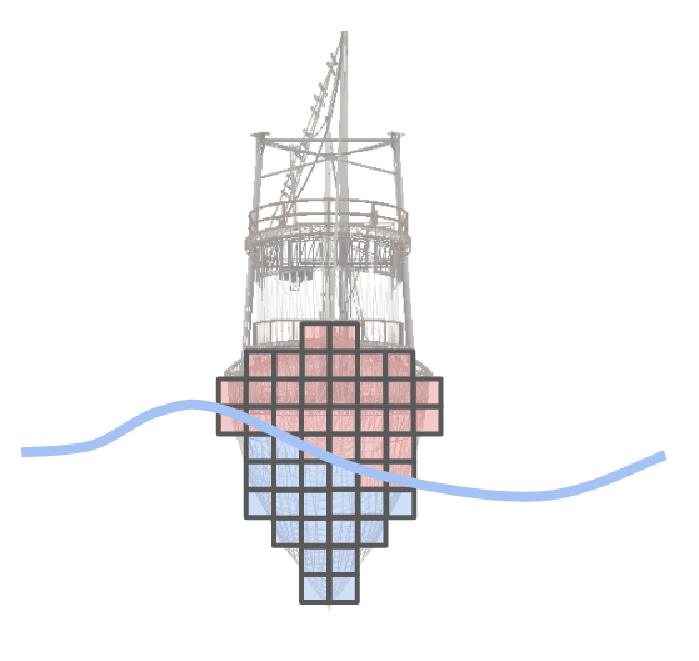
\includegraphics[width=\linewidth]{images/ship_algo_2.pdf}
  \caption{Computational grid divided into two parts: immersed (blue) and above water (red).}
  \label{fig:ship_algo_2}
\end{subfigure}\hfil % <-- added
\begin{subfigure}{0.25\textwidth}
  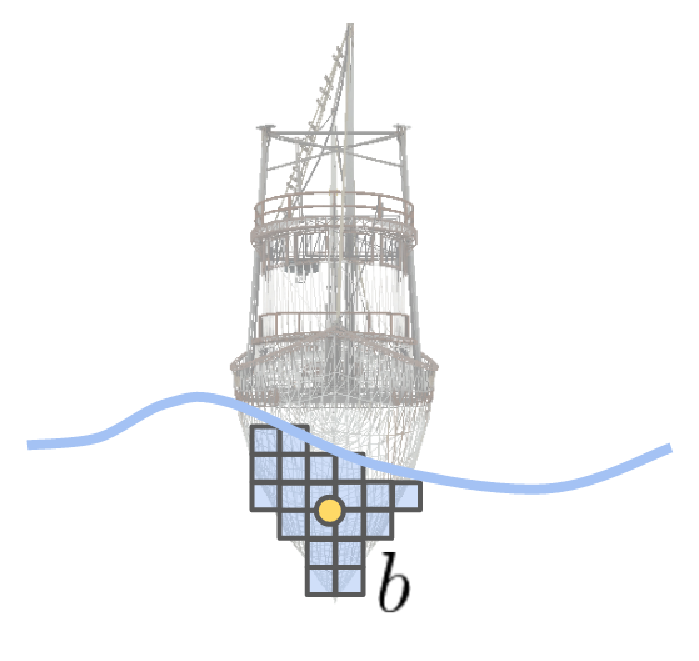
\includegraphics[width=\linewidth]{images/ship_algo_3.pdf}
  \caption{Buoyancy point $b$ estimated as a center of mass of immersed part.}
  \label{fig:ship_algo_3}
\end{subfigure}

\medskip
\begin{subfigure}{0.25\textwidth}
  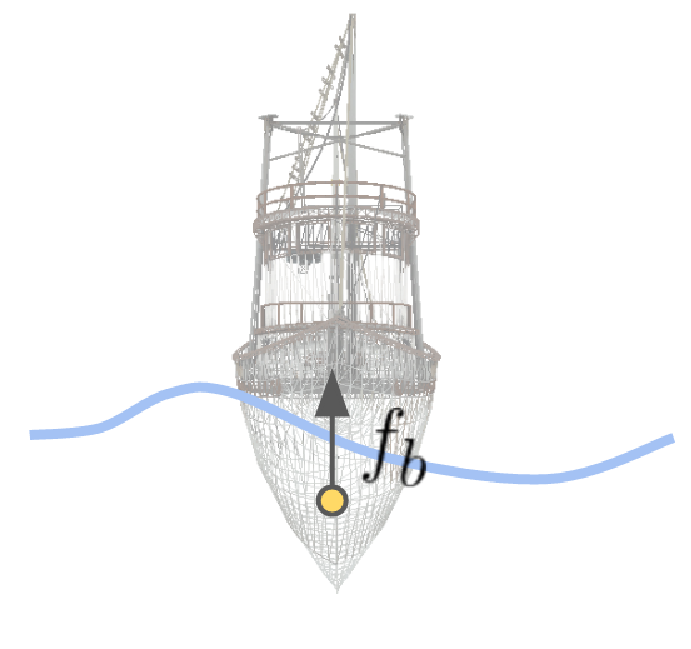
\includegraphics[width=\linewidth]{images/ship_algo_4.pdf}
  \caption{Buoyancy force $f_b$ at point $b$ computed using Archimedes principle formula.}
  \label{fig:ship_algo_4}
\end{subfigure}\hfil % <-- added
\begin{subfigure}{0.25\textwidth}
  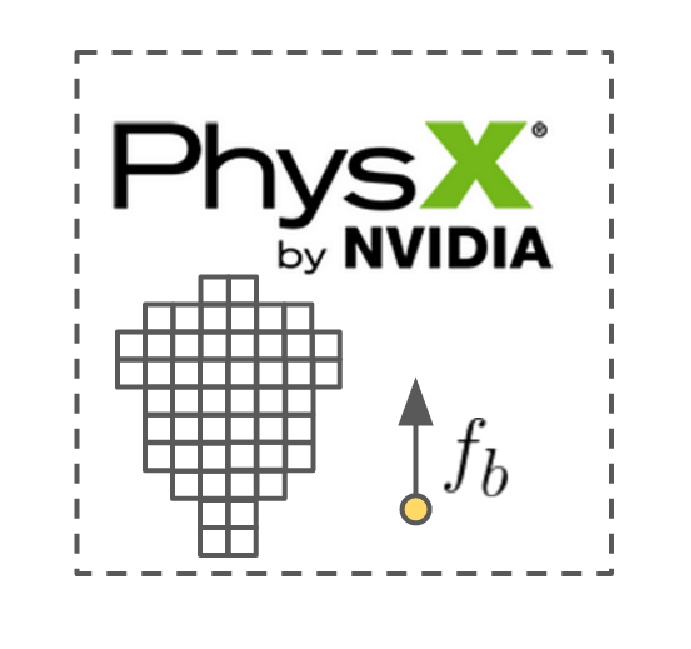
\includegraphics[width=\linewidth]{images/ship_algo_5.pdf}
  \caption{PhysX library using $f_b$ and its own copy of computational grid computes transformations.}
  \label{fig:ship_algo_5}
\end{subfigure}\hfil % <-- added
\begin{subfigure}{0.25\textwidth}
  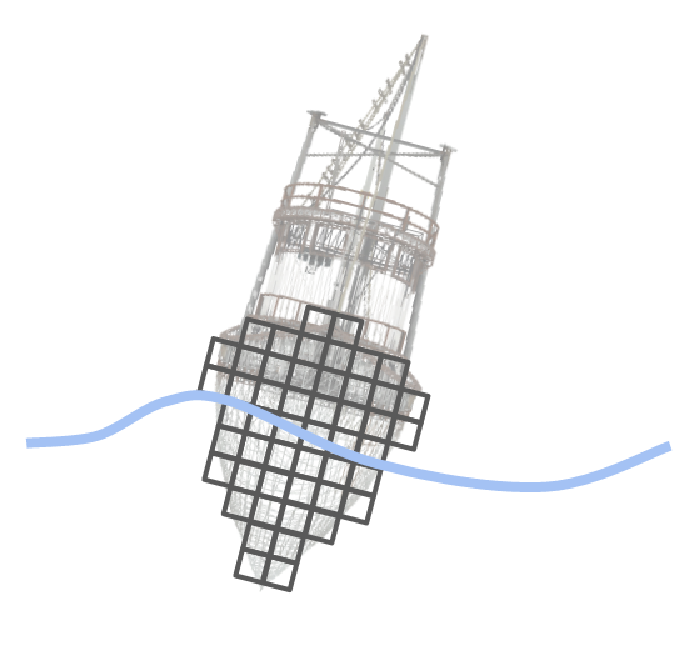
\includegraphics[width=\linewidth]{images/ship_algo_6.pdf}
  \caption{Transformations computed by PhysX library applied to computational grid and the ship's model.}
  \label{fig:ship_algo_6}
\end{subfigure}
\caption{Overview of the simulation algorithm flow.}
\label{fig:images}
\end{figure}

\subsubsection{Immersed Part of the Ship}
As a consequence of water movement, some part of the ship's computational grid might be treated as "immersed" i.e. located under the water surface. The project assumes that state of immersion is not binary one. A cell can be immersed partially, which forces one to calculates its under-water volume. Let us assume that a cell of width $c_w$ and volume $v_c$, has its center at $c=(x_x, c_y, c_z)$. Using water height field and cells center one can estimate level of immersion using following equation:
\begin{equation}\label{eq:immersion}
    v_{immersed} = 
    \begin{cases}
        (\frac{h_{sea} - c_y}{c_w} + 0.5)\cdot v_c,& c_y - h_{sea} \leqslant \frac{c_w}{2}\\
        0 ,              & \text{otherwise}
    \end{cases}
\end{equation}

where $h_{sea}$ is a level of the water for a given cell. The level is calculated as a closest vertex of the water grid in a cell center's neighbourhood. Note, that if $c_y - h_{sea} > \frac{c_w}{2}$ then cell is considered: not-immersed, hence its $v_{immersed} = 0$.

\subsubsection{Buoyancy Center $b$}
Method presented in the section is taken form \cite{second_paper}. First, let assume that buoyancy center has been defined as $b = (x_b, y_b, z_b)$, where $b \in \mathbb{R}^3$. To compute its x-axis component ($x_b$) all immersed cells with the same x coordinates should be grouped in so-called slices. It will result in dividing the computational grid into $k$ cross-sections as presented on figure ??. Treating immersed part of a grid as a one dimensional beam, physical law for calculating beam's mass center can be used to estimate $x_b$ as follows:
\begin{equation}\label{eq:b_center}
x_b = (\Sigma_{i=1}^{k} \rho \cdot v_i \cdot x_i)  / m_s
\end{equation} 
where $\rho$ is sea water density, $v_i$ represents immersed part of ith slice (computed as a sum of immersed portions of cells in ith cross-section), $x_i$ is x-coordinate of the ith slice (in ship's local frame of reference) and $m_s$ represents total mass of computational grid. Equation \ref{eq:b_center} can be easily adapted to calculate other two $b$ components. 
\subsubsection{Buoyancy Force $f_b$}
To compute the force Archimedes' principle will be used. It indicates that the upward buoyant force that is exerted on a body immersed in a fluid, whether fully or partially submerged, is equal to the weight of the fluid that the body displaces \cite{arch}. Although the formula does not consider the surface tension (capillarity) acting on the body, it will suit the project's purposes. The equation is as follows:
\begin{equation}
f_b = \rho \cdot g \cdot v
\end{equation}
where $\rho$ represents water density, $g$ is an acceleration due to gravity and $v$ indicates volume of displaced water. In our case $v$ is sum of $v_{immersed}$ of every immersed cell of computational grid. 

\subsubsection{Behind PhysX Scenes} \label{subsub:physX}
Following section constitutes a short outline of calculations done by PhysX. Its purpose is to sketch a general idea about what is done to compute the grid transformations and one can find it useful in case of extending functionalities.

Once the library receives buoyancy force $f_b$ applied at buoyancy center $b$ it calculates the torque of the force with respect to the center of mass $g$ of the grid. Since PhysX stores cells positions, densities and masses it can easily compute $g$ by itself. Next step is to calculate moment of inertia tensor of the entire grid. Due to fact that the tensor will be calculated with respect to $g$ and object is composed of multiple cubes, following steps must be applied:  
\begin{enumerate}
\item Calculate each cube's moment of inertia tensor with respect to its center of mass.
\item Calculate each cube's moment of inertia tensor with respect to computational grid's center of mass.
\item Sum all inertia tensors to acquire computational grid's moment of inertia tensor.
\end{enumerate} 
First point is relatively easy due to fact that each cube has uniform density (not necessarily the same as others) and requires using widely know matrix:
\[
I_c=
  \begin{bmatrix}
    \frac{1}{6} \cdot c_m \cdot c_w & 0 & 0 \\
    0 & \frac{1}{6} \cdot c_m \cdot c_w & 0 \\
    0 & 0 & \frac{1}{6} \cdot c_m \cdot c_w
  \end{bmatrix}
\]
where $c_m$ is cube's mass and $c_w$ represents its width.

Next part involves using Steiner's formula, which defines a means for describing a dependency between moment of inertia with respect to an axis and other axis parallel to it. In our case a cube's center of mass axis is parallel to the grid's center of mass axis, hence the formula can be applied and it looks as follows:
\[
I_s = I_c + c_m \cdot (c_c-g)^{2}
\]
where $I_s$ and $I_c$ are inertia tensors of particular cube with respect to the grid's center of a mass and a cube's center of mass, respectively. $c_c$ is the center of mass of a cube, and $g$ indicates center of mass of the grid. In the project's case (three dimensional tensors), assuming that $(c_c - g) = (x, y, z)$:
\[
c_m \cdot (c_c-g)^{2} =
  \begin{bmatrix}
    (y^2 + z^2)c_m & -x y c_m & -x z c_m \\
    -x y c_m & (x^2 + z^2)c_m & -y z c_m \\
    -x z c_m  & -y z c_m & (x^2 + y^2)c_m
  \end{bmatrix}
\]
To acquire inertia tensor $I_g$ of entire grid, one needs to sum $I_s$ for each cube i.e. 
\[
I_g = \Sigma I_s
\]
Having $I_g$ and torque determined by $f_b$ and $b$, PhysX is able to estimate (and return in form of a matrix) all required transformations of the grid in a next time step of an animation.
%---------------------------------------------------------------
\newpage
\section{Modelling} \label{sec:model}
Following section contains UML diagrams of three main scene's objects: water grid, skybox and the ship model. All of them have a brief description  in order to give an intuition about the architecture. 

\subsection{Water Grid}
The water grid is composed of a grid geometry and renderable objects. It must be given an id of a cubemap texture in order to shade its surface correctly. Internal \texttt{CWavesDeformer} class is responsible for off-screen rendering. Due to polymorphism, it can be casted onto its parent class (\texttt{CRenderableObject}) and packed with other objects that inherits after it. In such a solution one could iterate over data structure containing them and just call \texttt{render} function.

\begin{figure}[H]
    \centering
    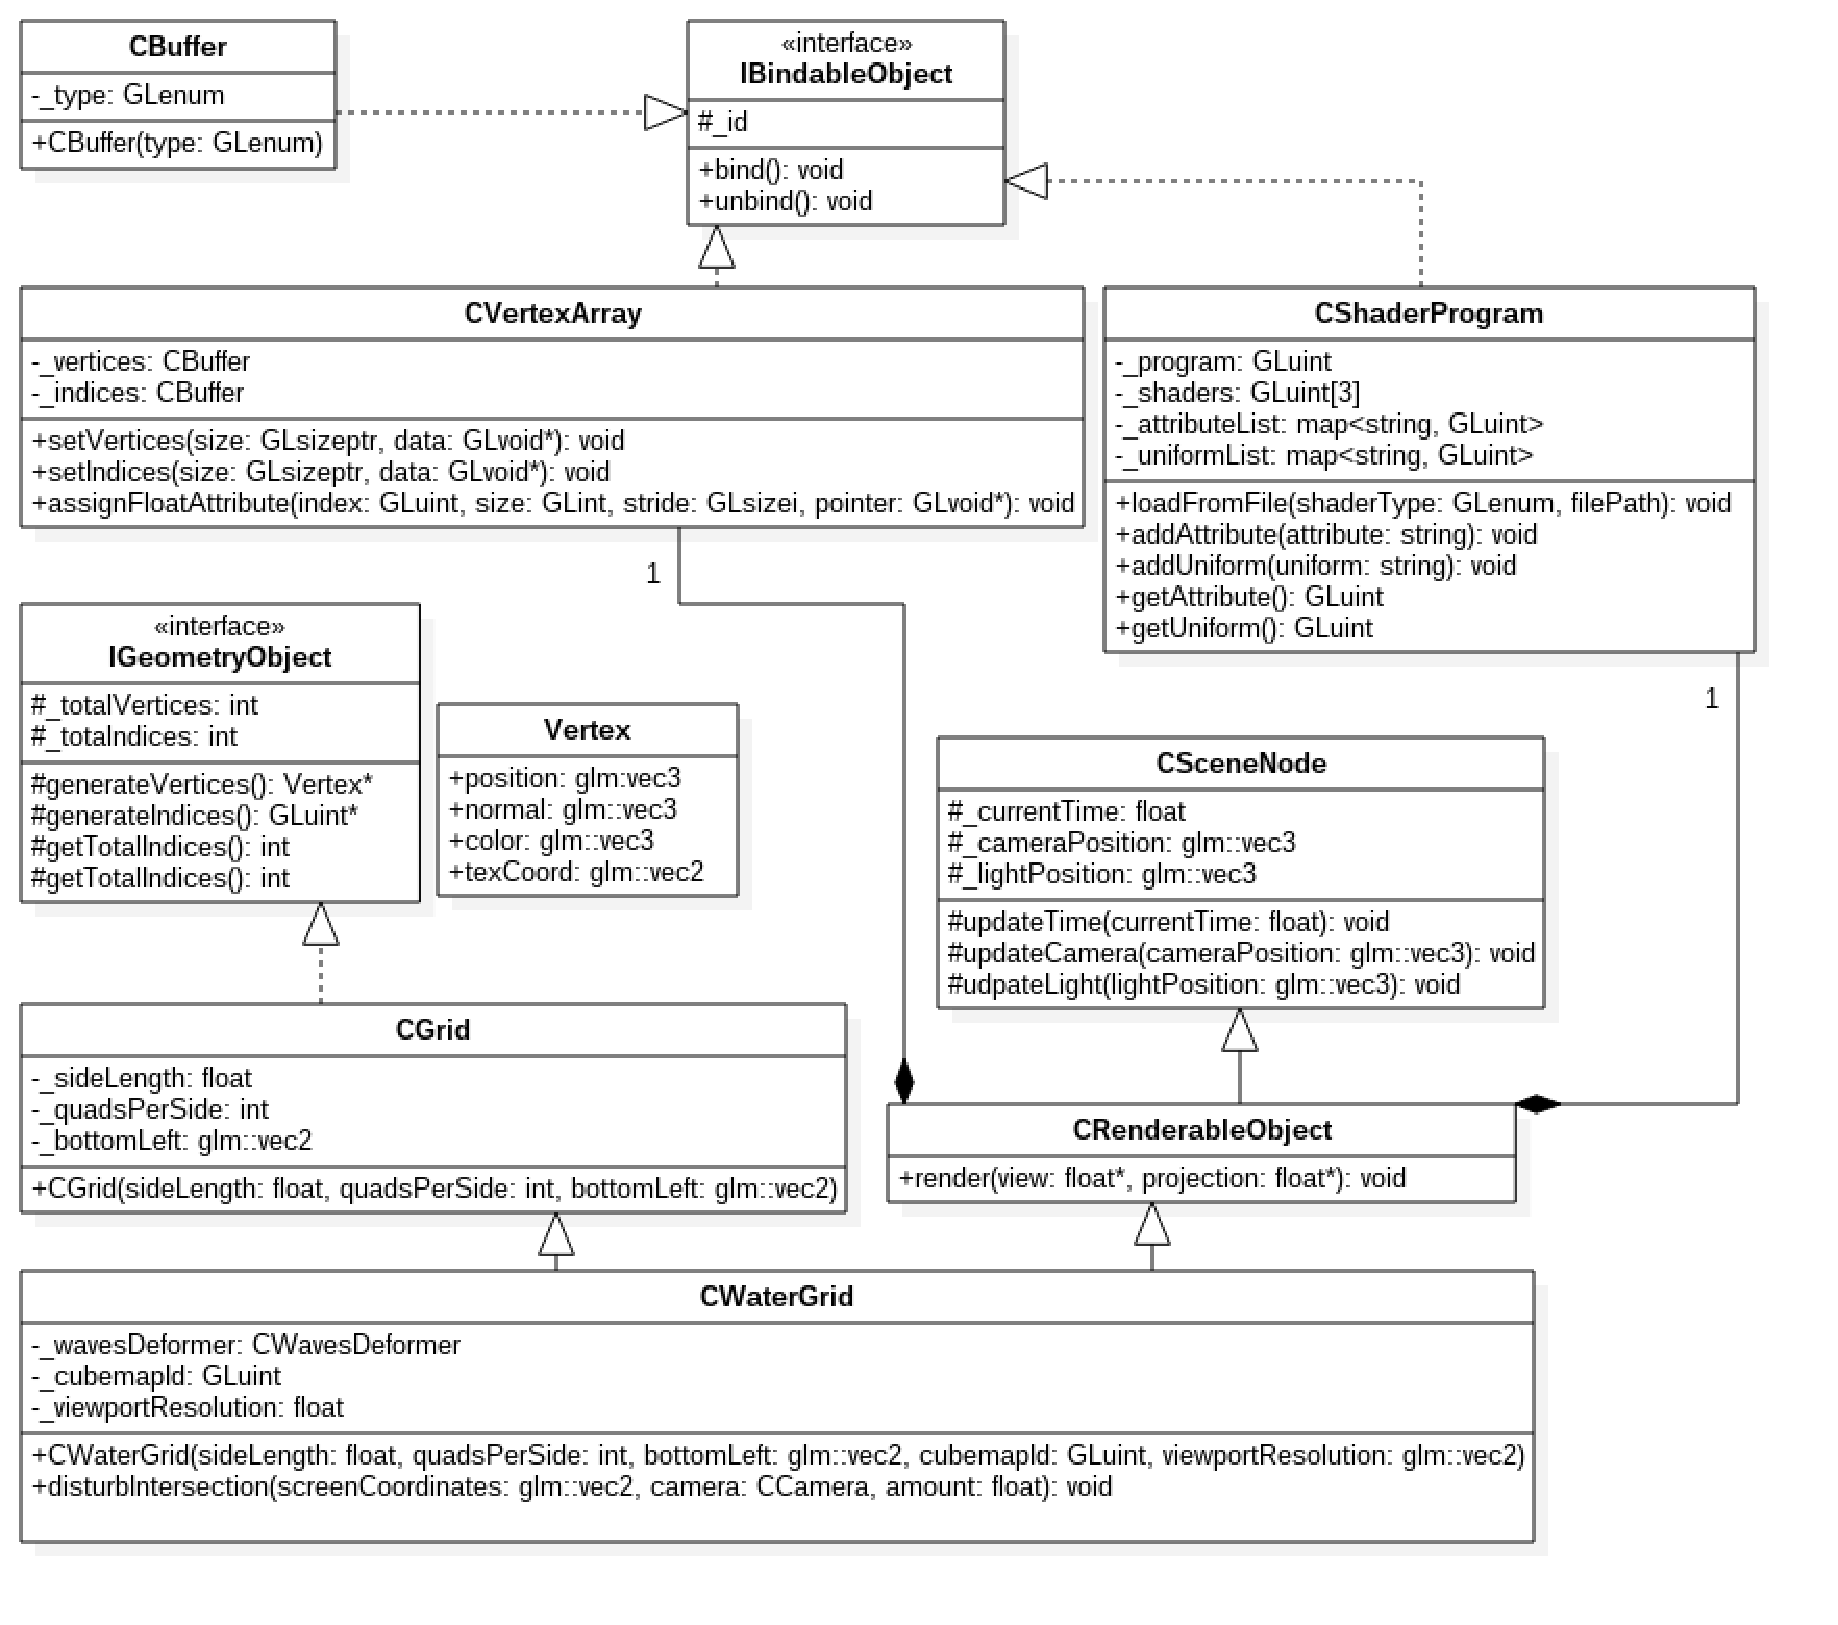
\includegraphics[width=1.0\textwidth]{images/water_grid_uml.pdf}
    \caption{Class diagram of CWaterGrid class.}
    \label{fig:water_grid_uml}
\end{figure}

\newpage
\subsection{Skybox}
The skybox is strictly dependent on two factors: water grid's side length and six paths to images that will constitute its faces. Its \texttt{getCubemapId} function is vital for the grid class. 
\begin{figure}[H]
    \centering
    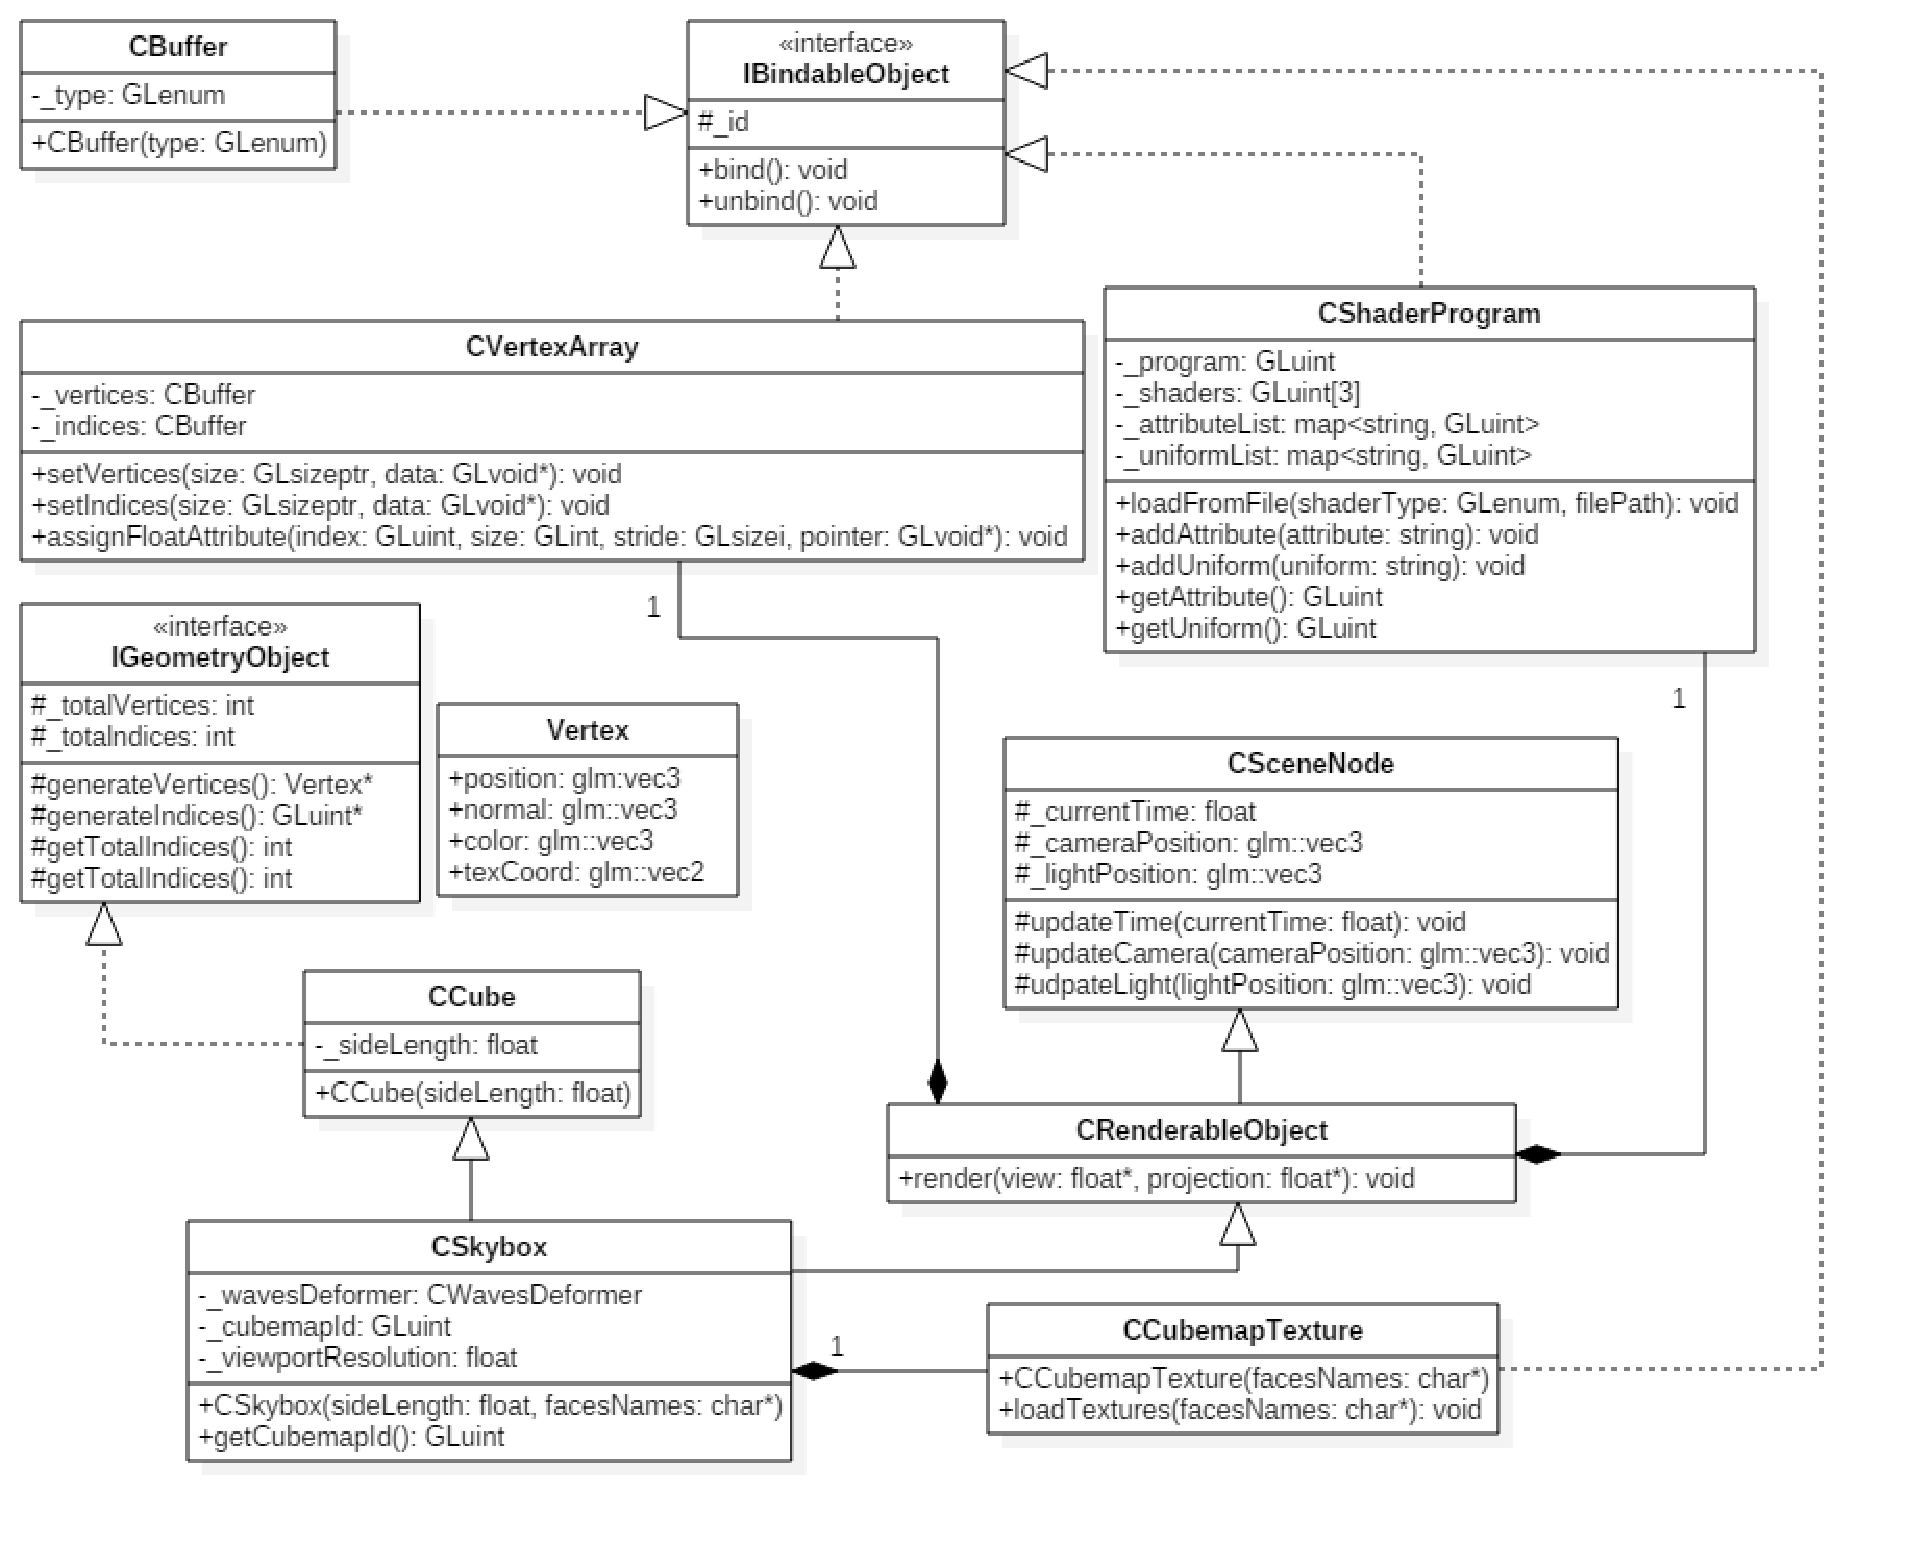
\includegraphics[width=1.0\textwidth]{images/skybox_uml.pdf}
    \caption{Class diagram of CSkybox class.}
    \label{fig:skybox_uml}
\end{figure}

\newpage
\subsection{Ship Model}
Ship model a little bit differs from other two main components. It is because its mesh is based solely on loaded .obj file, rather than predefined geometry. The class takes a path to the model file and via its \texttt{setModelMatrix}, position within scene can be set.
\begin{figure}[H]
    \centering
    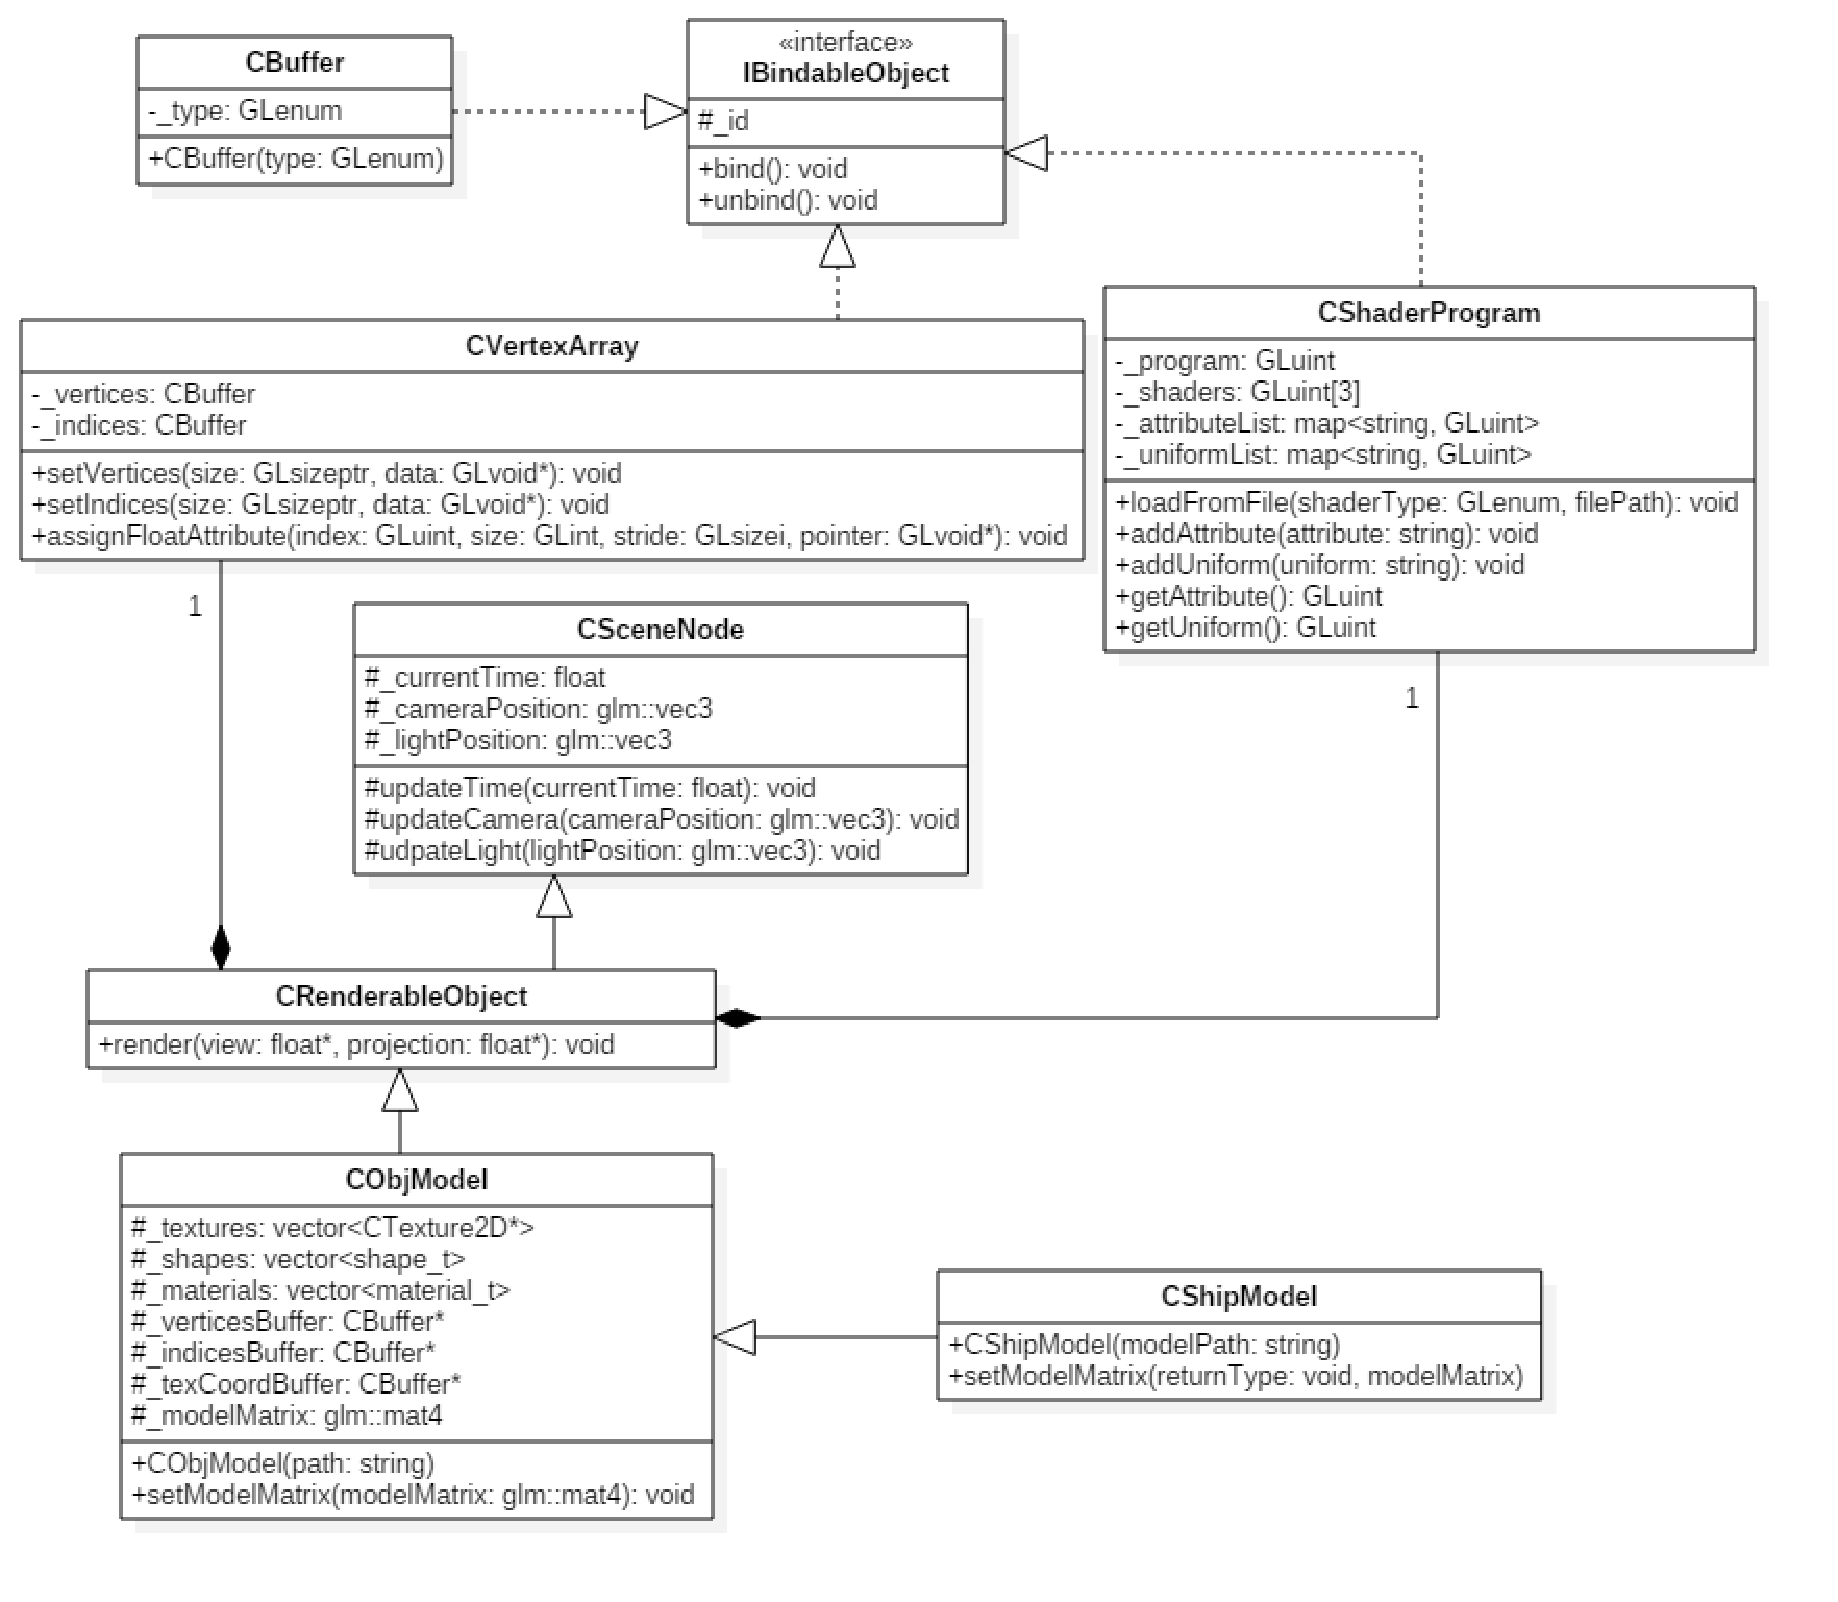
\includegraphics[width=1.0\textwidth]{images/ship_model_uml.pdf}
    \caption{Class diagram of CShipModel class.}
    \label{fig:ship_model_uml}
\end{figure}

\pagebreak
\section{Tests Design}
\subsection{Unit Tests}
Tests listed below will check the application's code. They will determine if various procedures behave correctly. Both returned values and internal actions will be checked.

\subsubsection{Application Namespace}
\begin{itemize}
	
%
% CGLFWRenderer
%
\item \texttt{class CGLFWRenderer}
		\begin{itemize}
			\item Method \texttt{\_initGLFW} initializes GLFW context without any errors
			\item Method \texttt{\_initWindow} initializes a window without any errors
			\item Method \texttt{\_initInputOutput} initializes \_inputOutput private member without any errors
			\item Method \texttt{\_initGLEW} initializes GLEW context without any errors
			\item Method \texttt{\_initATWBar} initializes AntTweakBar elements without any errors
			\item Method \texttt{\_initCallbacks} initializes GLFW's callbacks without any error
			\item Method \texttt{\_initRenderableObjects} initializes \_skybox,  \_water and \_ship private members without any errors
		\end{itemize}
		
%
% CATWGui
%
\item \texttt{class CAtwGui}
		\begin{itemize}
			\item Method \texttt{initializeATW} initializes AntTweakBar context without any errors
			\item Method \texttt{initializeWaterBar} initializes a portion of GUI related to the water simulation management without any errors
			\item Method \texttt{initializeSceneBar} initializes a portion of GUI related to the general application management without any errors
			\item Method \texttt{initializeShipBar} initializes a portion of GUI related to the ship simulation management without any errors
			\item Method \texttt{initializeControlsBar} initializes a portion of GUI related to the application controls information without any errors
			\item Method \texttt{terminateATW} terminates AntTweakBar context without any errors
			\item Method \texttt{getDisturbanceHeight} returns current strength of per-vertex disturbance
			\item Method \texttt{getKernelSize} returns current size of disturbance's kernel.
			\item Method \texttt{getFlatness} returns current value of  disturbance's flatness coefficient.
			\item Method \texttt{getIsRaining} returns a value indicating whether rain simulation should be active or not
			\item Method \texttt{getRainingIntensity} returns value indicating how often should disturbances caused by a rain occur.
			\item Method \texttt{getRainDropSize} returns value indicating how strong should disturbances caused by a rain be.	
			\item Method \texttt{getLightOn} returns a value indicating whether scene's lightening should be active or not		
			\item Method \texttt{getLightDirection} returns a vector representing current direction of a scene's light.
			\item Method \texttt{getWaterAnimation} returns a value indicating whether water animation should be active or not	
			\item Method \texttt{getComputationalGridOn} returns a value indicating whether computational grid should be displayed or not
		\end{itemize}
		
%
% CCustomCamera
%	
\item \texttt{class CCustomCamera}
		\begin{itemize}
			\item Method \texttt{updateViewingAngles} modifies horizontal and vertical angles of the camera.
			\item Method \texttt{moveBackward} modifies position of the camera moving it backward
			\item Method \texttt{moveLeft} modifies position of the camera moving it to the left
			\item Method \texttt{moveRight} modifies position of the camera moving it to the right
			\item Method \texttt{moveUp} modifies position of the camera moving it up
			\item Method \texttt{moveDown} modifies position of the camera moving it down
			\item Method \texttt{getProjectionMatrix} returns correct \textit{perspective} matrix with respect to the camera settings
			\item Method \texttt{getViewMatrix} returns correct \textit{lookAt} matrix with respect to the camera settings
			\item Method \texttt{getDirectionVector} returns correct vector with camera direction.
			\item Method \texttt{getUpVector} returns correct vector that is a result of cross product of camera's right vector and direction vector.
			\item Method \texttt{getRightVector} returns correct vector that is perpendicular to the camera's up vector and points to the right with respect to direction vector
			\item Method \texttt{getPosition} returns correct camera's position
			\item Method \texttt{getVerticalAngle} returns correct camera's vertical angle	
			\item Method \texttt{getHorizontalAngle} returns correct camera's horizontal angle	
		\end{itemize}
%
% CGLFWInputOutput
%	
\item \texttt{class CGLFWInputOutput}
		\begin{itemize}
			\item Method \texttt{setCamera} updates \_camera field with a pointer to the camera object
			\item Method \texttt{setShip} updates \_ship field with a pointer to the ships object		
			\item Method \texttt{updateTime} handles mouse and keyboard input - in case of tests just no error should appear 
			\item Methods \texttt{setIntersectionRequested} and \texttt{isIntersectionRequested} updates \_intersectionRequested field and returns it, respectively 
			\item Methods \texttt{setStopAnimationRequested} and \texttt{isStopAnimationRequested} updates \_stopAnimationRequested field and returns it, respectively
		\end{itemize}
%
% CTimer
%	
\item \texttt{class CTimer}
		\begin{itemize}
			\item Method \texttt{tick} returns elapsed time since last call or object creation
		\end{itemize}
\end{itemize}
\subsubsection{Entities Namespace}
\begin{itemize}
%
% CShipModel
%	
\item \texttt{class CShipModel}
		\begin{itemize}
			\item Method \texttt{updateComputationalGrid} modifies ship's transformations
		\end{itemize}
%
% CSkybox
%	
\item \texttt{class CSkybox}
		\begin{itemize}
			\item Method \texttt{setCameraPosition} updates current camera position
			\item Method \texttt{getCubemapId} returns cubemap's id in OpenGL context
		\end{itemize}		

%
% CWaterGrid
%	
\item \texttt{class CWaterGrid}
		\begin{itemize}
			\item Method \texttt{updateTime} updates \_currentTime field with current time 
			\item Method \texttt{setCameraPosition} updates current camera position
			\item Method \texttt{setLightDirections} updates direction of light applied to render the water surface
			\item Method \texttt{setAnimation} correctly modifies \_animation field
			\item Methods \texttt{setAnimation} and \texttt{getAnimation} updates \_animation field and returns it, respectively 
			\item Methods \texttt{setLightOn} and \texttt{getLightOn} updates \_lightOn field and returns it, respectively 
			\item Method \texttt{getVerticesPerSide} returns number of vertices per water grid's side

		\end{itemize}			
		
\end{itemize}

\subsubsection{Geometry Namespace}
\begin{itemize}

%
% CCube
%	
\item \texttt{class CCube}
		\begin{itemize}
			\item Method \texttt{generateVertices} returns correct set of vertices describing a cube
			\item Method \texttt{generateIndices} returns correct indexing for a cube's vertices
			\item Method \texttt{getTotalVertices} returns number of vertices in a cube
			\item Method \texttt{getTotalIndices} returns number of indices in a cube
		\end{itemize}


%
% CGrid
%	
\item \texttt{class CGrid}
		\begin{itemize}
			\item Method \texttt{generateVertices} returns correct set of vertices describing a grid
			\item Method \texttt{generateIndices} returns correct indexing for a grid's vertices
			\item Method \texttt{getTotalVertices} returns number of vertices in a grid
			\item Method \texttt{getTotalIndices} returns number of indices in a grid
		\end{itemize}
		
		
%
% CQuad
%	
\item \texttt{class CQuad}
		\begin{itemize}
			\item Method \texttt{generateVertices} returns correct set of vertices describing a quad
			\item Method \texttt{generateIndices} returns correct indexing for a quad's vertices
			\item Method \texttt{getTotalVertices} returns number of vertices in a quad
			\item Method \texttt{getTotalIndices} returns number of indices in a quad
		\end{itemize}

%
% COBJModel
%	
\item \texttt{class COBJModel}
		\begin{itemize}
			\item Method \texttt{\_loadShapesAndMaterials} fills \_shapes and \_materials with appropriate data from .obj file
			\item Method \texttt{\_createTexturesFromImages} based on loaded materials creates textures without any errors
			\item Method \texttt{\_createBuffers} fills vertex array object with 3 distinct buffers concerning vertices, indices and textures coordinates
			\item Method \texttt{\_loadDataToBuffers} fills vertices, indices and textures coordinates buffers with data loaded from .obj file
			\item Method \texttt{\_initializeShaderProgram} links and compile shader program without any errors
		\end{itemize}	
		
\end{itemize}
\subsubsection{Rendering Namespace}
\begin{itemize}
%
% CBuffer
%	
\item \texttt{class CBuffer}
		\begin{itemize}
			\item Method \texttt{bind} binds buffer to the current OpenGL context without any errors
			\item Method \texttt{unbind} unbinds buffer to the current OpenGL context without any errors
			\item Method \texttt{setDataStatic} put provided data into buffer with GL\_STATIC\_DRAW without any errors
			\item Method \texttt{setSubData} updates a subset of buffer object's data without any errors
			\item Method \texttt{setDataStream} put provided data into buffer with GLGL\_STREAM\_DRAW without any errors
		\end{itemize}

%
% CFrameBuffer
%	
\item \texttt{class CFrameBuffer}
		\begin{itemize}
			\item Method \texttt{bind} binds frame buffer to the current OpenGL context without any errors
			\item Method \texttt{unbind} unbinds frame buffer to the current OpenGL context without any errors
			\item Method \texttt{setColorAttachment} Attach texture to frame buffer object without any errors
		\end{itemize}
		

%
% CVertexArray
%	
\item \texttt{class CVertexArray}
		\begin{itemize}
			\item Method \texttt{bind} binds vertex array to the current OpenGL context without any errors
			\item Method \texttt{unbind} unbinds vertex array to the current OpenGL context without any errors
			\item Method \texttt{bindBuffers} binds all buffers attached to vertex array without any errors
			\item Method \texttt{unbindBuffers} unbinds all buffers attached to vertex array without any errors
			\item Method \texttt{setBuffer} adds a buffer of a given type to vertex array object
			\item Method \texttt{getBuffer} allows to access some particular buffer by its name
			\item Method \texttt{assignFloatAttribute} assignings shader's attribute to vertex array object without any errors
		\end{itemize}		
%
% CCubemapTexture
%	
\item \texttt{class CCubemapTexture}
		\begin{itemize}
			\item Method \texttt{bind} binds textures to current GL\_TEXTURE\_CUBE\_MAP object
			\item Method \texttt{unbind} unbinds textures from GL\_TEXTURE\_CUBE\_MAP object
			\item Method \texttt{loadTexture} loads 6 textures as a faces of the cubemap texture without any errors
			\item Method \texttt{getId} returns proper id of the cubemap texture in terms of OpenGL context
		\end{itemize}

%
% CTexture2D
%	
\item \texttt{class CTexture2D}
		\begin{itemize}
			\item Method \texttt{bind} binds texture to current GL\_TEXTURE\_2D object
			\item Method \texttt{unbind} unbinds texture from GL\_TEXTURE\_2D object
			\item Method \texttt{\_textureFromFile} loads texture from file
		\end{itemize}

%
% GLSLShader
%	
\item \texttt{class GLSLShader}
		\begin{itemize}
			\item Method \texttt{bind} binds shader to the current OpenGL context without any errors
			\item Method \texttt{unbind} unbinds shader to the current OpenGL context without any errors
			\item Method \texttt{loadFromFIle} loads shader from specified file
			\item Method \texttt{createAndLinkProgram} creates and links shader program without any errors from OpenGL context
			\item Method \texttt{addAttribute} adds attribute to shader's internal map of attributes
			\item Method \texttt{addUniform} adds uniform to shader's internal map of attributes
		\end{itemize}
		
\end{itemize}

\subsubsection{Utils Namespace}
\begin{itemize}
%
% class CWavesDeformer
%	
\item \texttt{class CWavesDeformer}
		\begin{itemize}
			\item Method \texttt{bindTexture} binds texture with next animation step data to the current texture unit within OpenGL context
			\item Method \texttt{bindTexture} unbinds texture with next animation step data to the current texture unit within OpenGL context
			\item Method \texttt{animationStep} performs next animation step's calculations
			\item Method \texttt{pointDisturbance} disturbs particular vertex by specified amount
			\item Method \texttt{areaDisturbance} disturbs particular vertex' neighbourhood with specified kernel, amount and flatness
		\end{itemize}

\item functions
		\begin{itemize}
			\item Function \texttt{randomInteger} returns random integer from specified interval
			\item Function \texttt{randomFloat} returns random float from specified interval
			\item Function \texttt{animationStep} performs next animation step's calculations
			\item Function \texttt{pointDisturbance} disturbs particular vertex by specified amount
			\item Function \texttt{toNormalizedDeviceCoordinates} transforms given point to normalized device coordinates
			\item Function \texttt{toCameraCoordinates} transforms given point from clip space to camera space
			\item Function \texttt{rayIntersectsPlane} determines whether given point intersects specified plane or not
			\item Function \texttt{readFromIni} loads data from specified .ini file
		\end{itemize}
		
\end{itemize}
\subsection{Acceptance Tests}
Following list includes different tests that are prepared to check the application's functionalities. One should note that not all of  existing graphical user interface options are assumed to be tested. It is caused by the fact that some buttons are purely auxiliary and were not specifically requested by the client.
\subsubsection{Camera Movement}
\begin{itemize}
\item User can look around the scene with usage of right mouse button
\item User can move around the scene with usage of following keys: w, s, a, d, z, x
\item There are no constraints regarding objects penetrating - e.g.  camera can be located inside ship hall.
\item Changing value of \textit{Scene/Camera/Speed/Movement} results in the camera's speed on the scene.
\item Changing value of \textit{Scene/Camera/Speed/Angular} impacts the camera's rotation speed.
\end{itemize}
\subsubsection{Interaction with the Water}
\begin{itemize}
\item Clicking on the water surface results in grid's disturbance
\item Nothing happens when one click somewhere else than the water surface
\item Disturbances have impact on ship model (computational grid detects changes in the grid's heights)
\item Value of \textit{Water/Manual\_Disturbance/Strength} increases disturbance height.
\item Value of \textit{Water/Manual\_Disturbance/Kernel} increases disturbance starting area.
\item Different values of\textit{Water/Manual\_Disturbance/Flatness} results in steeper disturbance shapes.
\end{itemize}
\subsubsection{Waves}
\begin{itemize}
\item Computational grid reacts on waves, causing the model to move.
\item Enabling/disabling \textit{Water/Waves/On Off} results in displaying and hiding random waves disturbance, respectively. 
\item Different values of \textit{Water/Waves/Amplitude} results in higher/lower waves.
\item Different values of \textit{Water/Waves/Frequency} results in faster and more frequent waves animation.
\end{itemize}
\subsubsection{The Ship}
\begin{itemize}
\item Pressing up and down arrow results in increasing and decreasing a force applied in the front of the ship's hull. As a results the model should move forward with different speed or stop.
\item Pressing left and right arrow results in increasing and decreasing a force applied in the front of the ship's hull, oriented to the west and east, respectively. As a results the model should turn left or right (depending on the force).
\item Enabling/disabling \textit{Ship/Simulation/Grid visible} results in displaying and hiding computational grid, respectively. The grid's cells should be black when are above water and blue if immersed.
\item \textit{X}, \textit{Y}, \textit{Z} values of \textit{Ship/Simulation/Local Translation} translates the model relatively to the computational grid.
\item Tweaking \textit{Ship/Simulation/Model Scale} affects the model size.
\item Values of \textit{Ship/Simulation/Linear Damping} and \textit{Ship/Simulation/Angular Damping} influences the model's stability in terms of the simulation. E.g. higher the value of angular damping, more stable the ship. 
\end{itemize}

\subsection{Tests Report}
All aforementioned tests have passed. I assume that they thoroughly check both: code and functionality of the application. In addition they cover every critical section of the simulation, hence can be seen as reliable. Unit tests were written with usage of Google Test framework, while the acceptance tests were performed with the executable shipped with the following work.

\section{User Manual}
The section will present how to build the application executable from the raw source files (Section \ref{sub:building}. In addition compiling the installation program and its manual are presented in sections \ref{sub:building_setup} and \ref{sub:using_setup}. Last but not least, complete graphical user interface documentation is located in section \ref{sub:gui_doc}.
\subsection{Building} \label{sub:building}
\subsubsection{The Application} \label{subsub:build_app}
Currently only Windows platform is supported. Sources have been compiled on Windows 10 64bit with usage of Microsoft Visual Studio 2015 (and only that combination is assured to work). 

The procedure itself is rather straight forward and assumes that one has installed:
\begin{itemize}
\item CMake in version at least 2.8.4
\item Microsoft Visual Studio 
\end{itemize}

Steps needed to compile the program:
\begin{enumerate}
\item In repository's main directory call following commands:
 \begin{lstlisting}
mkdir [project directory]
cd [project directory]
cmake ..
 \end{lstlisting}
\item Open  \textit{[repository main folder]/[project directory]/BachelorThesis.sln} solution with Microsoft Visual Studio.
\item Change \textit{Debug} to \textit{Release} and click Build $\rightarrow$ Build Solution.
\end{enumerate}
Right now folder \textit{[repository main folder]/[project directory]/Release} should contain \textit{bachelor\_water.exe}, which is the application's main executable.
\subsubsection{The Setup Program} \label{sub:building_setup}
The program's sources come with script that produces an installation program. One is required only to have \textit{Inno Setup Compiler} installed, which can be acquired for free from its author's webpage \cite{inno_setup}. 

In order to compile the setup executable:
\begin{enumerate}
\item Build the application using steps from section \ref{subsub:build_app}
\item Go to  \textit{[repository main folder]/[project directory]/Release/win\_installer}
\item Open and compile \textit{[main folder]/[project directory]/Release/win\_installer/win\_installer.iss} 
\end{enumerate}


Setup executable resides in:  \textit{[repository main folder]/[project directory]/Release/win\_installer/Output} 

\subsection{Installation} \label{sub:using_setup}
Assuming that one is using the installer - the process itself is really straightforward. First, one will be presented with a welcome screen that briefly describes what will happen in next few steps. Figure \ref{fig:installation_1} constitutes a screenshot from the application. Naturally button \textit{Next} should be selected. 
\begin{figure}[H] 
    \centering
    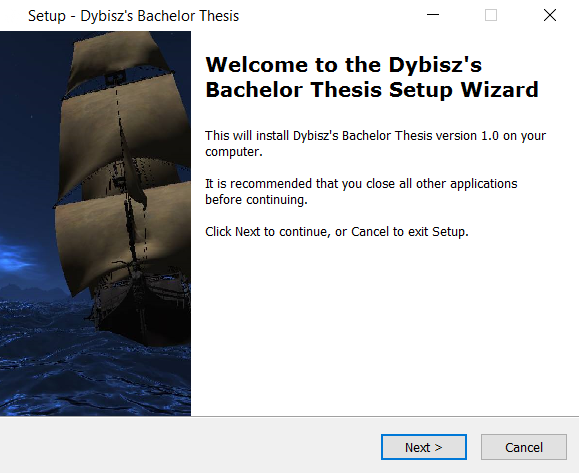
\includegraphics[width=0.5\textwidth]{images/installation_1.png}
    \caption{Welcome page of the setup program.}
    \label{fig:installation_1}
\end{figure}

Second step differs from machine to machine. The program will attempt to recognize one's system bitness and determine whether he or she has an appropriate redistributable. The latter will be based on two factors: a correct entry in registry and existance of \textit{mscvp140.dll} in the system. In case of missing libraries - the application will prompt warning massage (Figure  \ref{fig:installation_2_error}), otherwise one should see Figure \ref{fig:isntallation_2}. Note that the installer will provide missing libraries.

\begin{figure}[H]
\begin{subfigure}{.5\textwidth}
  \centering
  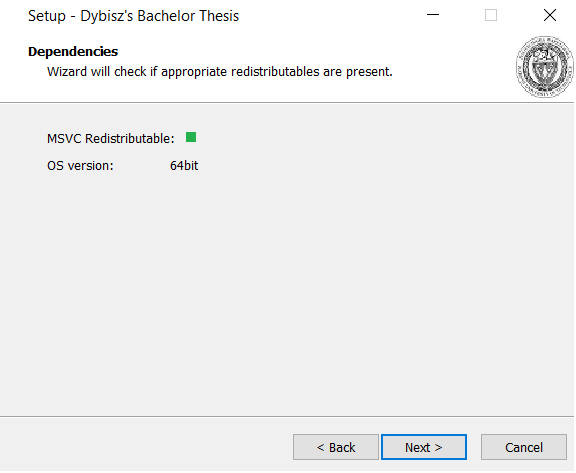
\includegraphics[width=.9\linewidth]{images/installation_2.png}
  \caption{Installation process on 64bit system that fulfills the requirements.}
  \label{fig:isntallation_2}
\end{subfigure}%
\begin{subfigure}{.5\textwidth}
  \centering
  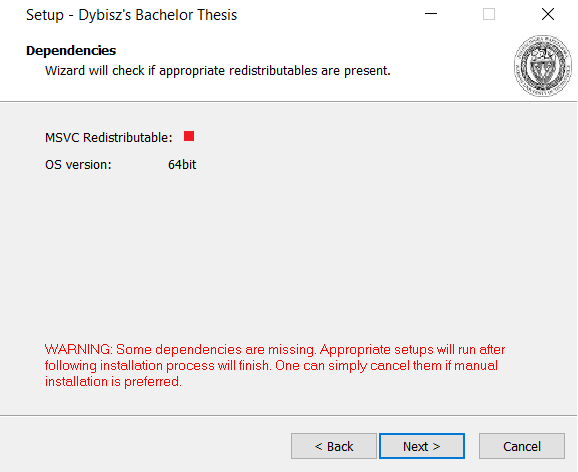
\includegraphics[width=.9\linewidth]{images/installation_2_error.png}
  \caption{Installation process on 64bit system without needed redistributables.}
  \label{fig:installation_2_error}
\end{subfigure}
\caption{Looking for redistributables}
\label{fig:installation_redists}
\end{figure}

Third step forces one to accept the license agreement. It is the MIT License, which allows a user to freely use, modify and distribute the source code, assuming that \textit{'The above copyright notice and this permission notice shall be included in all copies or substantial portions of the Software.'}. Standard open source license; Figure \ref{fig:isntallation_3}. Last step just informs that at this point the installation is ready. One should click \textit{Install} button and wait for the program to finish. Note that additional redistributables installers will pop up in case of missing libraries.

\begin{figure}[H]
\begin{subfigure}{.5\textwidth}
  \centering
  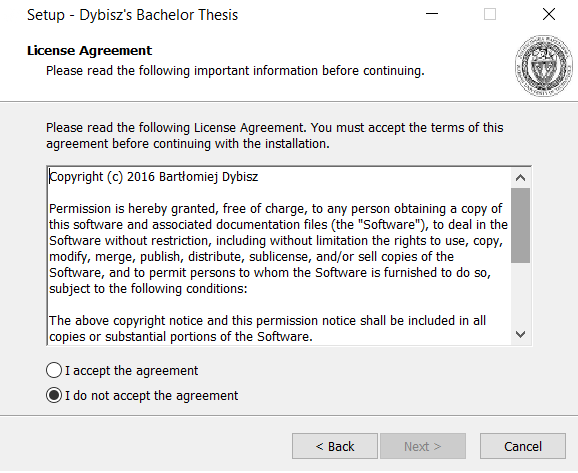
\includegraphics[width=.9\linewidth]{images/installation_3.png}
  \caption{License agreement.}
  \label{fig:isntallation_3}
\end{subfigure}%
\begin{subfigure}{.5\textwidth}
  \centering
  
\includegraphics[width=.9\linewidth]{images/installation_4.png}
  \caption{The last step.}
  \label{fig:sfig2}
\end{subfigure}
\label{fig:installation_4}
\end{figure}

\subsection{Graphical User Interface} \label{sub:gui_doc}
The interface (later referred to as GUI) is quite extensive. One is suggested to refer to Figure \ref{fig:gui_example} while reading. Generally, GUI is divided into 3 windows (Water, Scene and Ship) and one 'info box' with listed controls. Following section will briefly describe each of the windows fields. What is more, one should note that all of the following configurations are loaded directly from \textit{config.ini} file located in the executable directory.

\begin{figure}[H] 
    \centering
    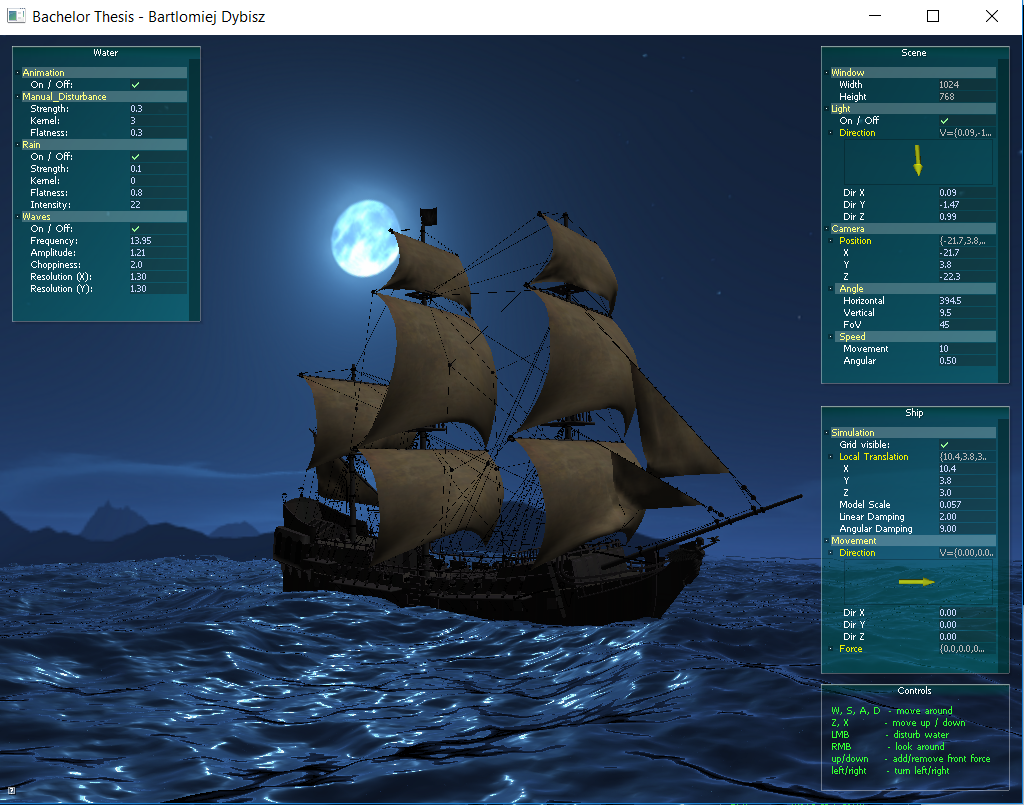
\includegraphics[width=0.75\textwidth]{images/gui_example.png}
    \caption{The application's graphical interface.}
    \label{fig:gui_example}
\end{figure}

\subsubsection{Water Window}
In charge of all movement related to the water's grid. It is by default located in the upper left corner of the screen.

\begin{itemize}
\item \texttt{[Animation: On / Off]} 

Freezes the water animation. Ship simulation will not be stopped.

\item \texttt{[Manual\_Disturbance: Strength]} 

Set height of the manual water disturbance. It will force more or less water to be displaced during LMB grid's disturbance.

\item \texttt{[Manual\_Disturbance: Kernel]} 

Each disturbance can involve more than one vertex. Following field specify the area that will be disturbed. E.g. value $3$ will mean $3x\times 3$ area, hence $9$ vertices will be disturbed.

\item \texttt{[Manual\_Disturbance: Flatness]} 

Area disturbance is based on $-a*(x^2 + y^2)$ function. The field sets value of $a$ - giving the function appropriate steepness.

\item \texttt{[Rain: On / Off]}

Turns on / off the rain, which is really a bunch of random disturbances along the grid. 

\item \texttt{[Rain: Strength]}

Height of each particular rain's disturbance. 

\item \texttt{[Rain: Kernel]}

Area of each particular rain's disturbance. See [Manual\_Disturbance: Kernel] for more information.

\item \texttt{[Rain: Flatness]}

Parameter's $a$ value of each particular rain's disturbance. See [Manual\_Disturbance: Flatness] for more information.

\item \texttt{[Rain: Intensity]}

How many random points per frame should be disturbed. Higher the value, more the rain 'drops' on the water surface.

\item \texttt{[Waves: On / Off]}

Turns on / off the grid's waves.

\item \texttt{[Waves: Frequency]}

Adjust frequency of the waves function. Higher values results in faster and more frequent waves.

\item \texttt{[Waves: Aplitude]}

Height of waves. 

\item \texttt{[Waves: Choppiness]}

Adjusts steepness of waves.

\item \texttt{[Waves: Resolution (X)]}

Stretches or shrinks the waves function along $X$ axis.

\item \texttt{[Waves: Resolution (Y)]}

Stretches or shrinks  the waves function along $Y$ axis.
\end{itemize}


\subsubsection{Scene Window}
\begin{itemize}
\item \texttt{[Window: Width]}

Constant that displays the scenes resolution width; cannot be modified.

\item \texttt{[Window: Height]}

Constant that displays the scenes resolution height; cannot be modified.

\item \texttt{[Light: On / Off]}

Turns on / off the water directional lightening.

\item \texttt{[Light: Direction]}

Since both, the water and the ship are shaded with directional light, GUI allows one to change its direction in real time. One is suggested to either tweak the $x$, $y$, $z$ components separately or use the arrow.

\item \texttt{[Camera: Position]}

Current camera location in the 3D space. Updated when using keyboard or 
can be manually set.

\item \texttt{[Camera: Angle]}

Horizontal and Vertical angles of the camera. Updated when using keyboard or can be set manually.

\item \texttt{[Camera: Speed]}

How fast should the camera travel each frame?

\end{itemize}
\subsubsection{Scene Window}
\begin{itemize}
\item \texttt{[Simulation: Grid visible]}

If on, three dimensional, computational grid will be rendered. What is more, immersed cells will be blue, while those above the water surface will be black.

\item \texttt{[Simulation: Local Translation]}

The model translation relative to the computational grid.

\item \texttt{[Simulation: Model Scale]}

How big should model be?

\item \texttt{[Simulation: Linear Damping]}

PhysX's damping of linear velocity.

\item \texttt{[Simulation: Angular Damping]}

PhysX's damping of angular velocity.

\item \texttt{[Movement: Direction]}

Can be set only via keyboard (up/down and left/right keys). 
Describes ship's movement force.
\end{itemize}

\section{Summary}
Project took more time than expected but all main requirements of the business analysis were met. In addition, auxiliary functionalities like e.g. water waves, basic rain or light were developed in order to make the scene more flexible and real-life looking. 

Although various supplementary features were presented there is still a room for more. One of the future enhancement might be e.g. alternative water shading, where each of six sides of the skybox would be based on off-screen rendered textures. Such an approach allows one to introduce surrounding rocks (cliffs) that would be reflected in the water. As an another example, one could make the disturbance equation more accurate by extending it with more components of Taylor's series. In addition, there is no doubt that flexibility of GUI might be developed via dynamic loading of configuration file, models and textures.

Source code has been prepared in a very flexible fashion, allowing one to easily transform the application into a computer game. Introducing new objects based either on primitive shapes or loaded models is rather uncomplicated and due to appropriate class hierarchy, OpenGL calls are encapsulated within objects that handle them. In a result, standard 'wall of code' of low-level calls is spread and hidden, positively influencing the transitivity of the sources.


%---------------------------------------------------------------
%\section{Bibliography}

\begin{thebibliography}{1}
\bibitem{gloss_1} \texttt{http://www.cise.ufl.edu/fishwick/introsim/node1.html}
\bibitem{gloss_2} \texttt{http://goanna.cs.rmit.edu.au/gl/teaching/rtr\&3dgp/notes/pipeline.html}
\bibitem{gloss_3} \texttt{http://www.gamedev.net/page/resources/\_/technical/graphics-programming-and-theory/introduction-to-the-graphics-pipeline-r3344}
\bibitem{gloss_4} \texttt{http://searchsoa.techtarget.com/definition/user-interface}
\bibitem{gloss_5} \texttt{https://unity3d.com/learn/tutorials/modules/beginner/graphics/using-skyboxes}
\bibitem{gloss_6} \texttt{http://findwords.info/term/heightmap}
\bibitem{physx} \texttt{https://developer.nvidia.com/physx-sdk}
\bibitem{anttweakbar} \texttt{http://anttweakbar.sourceforge.net/doc/}
\bibitem{soil} \texttt{http://www.lonesock.net/soil.html}
\bibitem{glew} \texttt{http://glew.sourceforge.net/}
\bibitem{glfw} \texttt{http://www.glfw.org/}
\bibitem{glm} \texttt{http://glm.g-truc.net/0.9.7/index.html}
\bibitem{inih} \texttt{https://github.com/benhoyt/inih}
\bibitem{scrum_definition} \texttt{https://www.techopedia.com/definition/13686/scrum}
\bibitem{scrum_guide} \texttt{http://www.scrumguides.org/scrum-guide.html}
\bibitem{shader_seascape} \texttt{https://www.shadertoy.com/view/Ms2SD1}
\bibitem{boat_source} \texttt{http://archive3d.net/?a=download\&id=78c1dca4}
\bibitem{gl_tutorial} \texttt{http://www.opengl-tutorial.org/beginners-tutorials/tutorial-3-matrices/}
\bibitem{gomez} M. Gomez, “Interactive Simulation of Water Surfaces”, Game Programming Gems Vol. 1, 2000
\bibitem{second_paper} S.-K. Ueng, “Physical models for simulation ship stability and hydrostatic motions”, Journal of

Marine Science and Technology, Vol. 21, No. 6, pp.674-685, 2013
\bibitem{arch} \texttt{http://formulas.tutorvista.com/physics/archimedes-principle-formula.html}

\bibitem{inno_setup} \texttt{http://www.jrsoftware.org/}
\end{thebibliography}
\end{document}


